% Hoda Abbasi
% 13 May 2016

\documentclass{report}
\input Latex_macros/Definitionen.tex

\usepackage{a4}
\usepackage{graphicx}
\usepackage{tikz-qtree}
\usepackage[active]{srcltx}
\usepackage[all]{xy}
\usepackage{enumerate}

\nc{\Dt}[1]{\mc{F}_{#1}} 
\nc{\tsubres}{\xrightarrow{\text{sfsR}}}
\nc{\tsubresk}[1]{\xrightarrow{\text{sfsR}}_{\!#1}}
\DMO{\saturate}{S}

\begin{document}
\title{Thesis Proposal: The combinatorics of minimally unsatisfiable clause-sets
       }

\author{Hoda Abbasi\\
        PhD Candidate\\
        Computer Science Department\\
        Swansea University\\}
\maketitle

%%%%%%%%%%%%%%%%%%%%%%%%%%%%%%%%%%%%%%%%%%%%%%%%%%%%%%%%%%

\begin{abstract}
This research investigates the connection between SAT problems (and particularly unsatisfiable problems) and combinatorics from two different aspects. The first aspect is concerned with two measures of resolution proof complexity. In general, there are various measures for representing the complexity of SAT problems called "hardness measures''. Here, two measures of hardness for resolution proofs ("tree-hardness'' and "width-hardness'') are reviewed and a game characterisation is investigated for them. This game is performed by two players for a clause-set $F$ and has an "optimal value'' corresponds to the hardness measures of $F$. Then, this game is applied for an special graphs called Tseitin graph to obtain the hardness measures.

The second aim of this research is to study the structure of minimally unsatisfiable clause-sets due to understand unsatisfiability. For investigating the properties of these clause-sets special reduction/extension are reviewed. Then, "deficiency" (the difference between the number of clauses and the number of variables in $F$) is used as a measure to classify minimally unsatisfiable clause-sets. So far, the structure of minimally unsatisfiable clause-sets with deficiency 1,2 are almost well-known but for higher deficiencies, our knowledge is limited. On the other hand, according to the literature it seems that there are finitely many-patterns for these clause-sets which is a motivation for further studies.
\end{abstract}

\tableofcontents
%%%%%%%%%%%%%%%%%%%%%%%%%%%%%%%%%%%%%%%%%%%%%%%%%%%%%%%%%%
\chapter{Introduction}
\label{cha:intro}

?????????

The hardness is defined as a measure of complexity (the amount of effort needed to discover unsatisfiability) for a representation $F$ of a boolean function $f$ in SAT solving. Various hardness measures have been investigated in the literature and the relation between these measures is studied in \cite{BeyersdorffGwynneKullmann2013PHPER,BeyersdorffKullmann2014PHP,GwynneKullmann2013GoodRepresentationsIIex}. In this proposal, two measures of the hardness are investigated. The first one is the tree-hardness which is related to the size of resolution proofs. The width-hardness is the second measure and is related to the width of clauses in resolution proofs. We start with defining these measures for unsatisfiable clause-sets and then, we extend the definitions to the satisfiable clause-sets. An overview of these two measure is given in \cite{BeyersdorffGwynneKullmann2013PHPER,BeyersdorffKullmann2014PHP,?? }.

For representing a boolean function $f$ CNF-clause-sets are defined in Section \ref{sec:Clause-sets}. Here, another representation of $f$ is introduced (called XOR-representation) which is used for extending the hardness game for graphs based on \cite{GwynneKullmann2013GoodRepresentationsIIex,GwynneKullmann2013GoodRepresentationsIILata}. An XOR-clause-set for $f$ is the interpretation of a clause-set $F \in \Cls$ as a system of XOR-constraints whose clauses $C$ are parity equation for $v \in \var(C)$. 
????
The XOR-representation is investigated in \cite{GwynneKullmann2013GoodRepresentations,GwynneKullmann2013GoodRepresentationsIIex,GwynneKullmann2013GoodRepresentationsIILata} with the goal of finding a good representation for XOR-constraints.
???????

One of the main class of unsatisfiable clause-sets are minimally unsatisfiable clause-sets which are referred as the building block for understanding unsatisfiability in \cite{KullmannZhao2010Extremal}. So, understanding the concept of minimally unsatisfiable clause-sets and investigating their properties and subclasses are important. An overview of these clause-sets are presented in \cite{KullmannZhao2010Extremal, Kullmann2007HandbuchMU,KullmannZhao2012ConfluenceJ}. An interesting measure for the complexity of clause-sets and particularly minimally unsatisfiable clause-sets is deficiency and it is used for classification of minimally unsatisfiable clause-sets. In Section \ref{cha:mucls}, first we give an overview of result regarding clause-sets with small deficiency and then, we discuss open problems and our research themes. So far, the structure of clause-sets in $\Musati{\delta=1}$ is well-known and an overview of them is given in \cite{KullmannZhao2010Extremal, Ku99dK,KleineBuening2000SubclassesMU,DDK98}. For clause-sets in $\Musati{\delta=2}$, \cite{KleineBuening2000SubclassesMU} gives a formula which is isomorphism for each $F' \in \Smusati{\delta=2}$ and further investigation on these clause-sets is presented in \cite{KullmannZhao2010Extremal, KleineBuening2000SubclassesMU, KullmannZhao2012ConfluenceJ}. The knowledge for the structure of clause-sets in $\Musati{\delta \ge 3}$ is very limited. For example, \cite{KullmannZhao2016UHitSAT} studies the characterization of clause-sets in $\Uclashi{\delta=2} \subset \Musati{\delta=2}$ and \cite{KullmannZhao2010Extremal} investigates some properties of clause-sets with deficiency three. Thus, characterization of clause-sets in this subclass is an open research question.

Some of first results in this report:

In chapter three:

In chapter four: 

The second chapter is dedicated to explain basic concepts and preliminaries. In chapter three, two hardness measures of clause-sets are introduced. Then, they are characterised by a game. Afterwards, the Tseitin clause-set (which is obtained from the Tseitin graph) is explained and the game is applied to them in order to obtain the hardness. Finally, ???

Chapter four explains ?????????



The initial results regarding the hardness measures in Chapter \ref{cha:Hd-TseitinG} are as follows:
  \begin{enumerate}
  \item Definition \ref{def:var-trb}: new definitions of trouble maker variables and ineffective variables.
  \item Definition \ref{def:atomicm}: a modified definition for the atomic move in game characterisation of the hardness.
  \item Lemma \ref{lem:atm-m-D-P}: the optimal atomic move in game characterisation of the hardness.
  \item Lemma \ref{lem:hd-game-main} and Lemma \ref{lem:gameres1}: a modified version of the asymmetric Prover-Delayer game to obtain the hardness of a clause-set $F \in \Cls$ based on the optimal atomic move.
  \item Lemma \ref{}: investigation of hardness change????????the effect of applying the sequence of partial assignment on the hardness of the initial clause-set????? during the game
  \item Lemma \ref{lem:game3}: investigation of the effect removing an edge on distribution of charges in a Tseitin graph.
  \item Lemma \ref{lem:game-tree}: characterisation of the game-tree for application of the hardness game for a Tseitin graph.
  \item Example \ref{exp:gg1}: the game-tree for the Tseitin graphs $K_3$.
  \item Lemma \ref{lem:tseitin-game-bridge}: the optimal atomic move for each players in the presence of a bridge in a Tseitin graph.
  \item Lemma \ref{lem:hd1hd2}: the effect of removing a bridge on the hardness of a Tseitin graph.
  \item Lemma \ref{lem:troubllemk-hd}: application of the definitions of trouble maker variable for a Tseitin graph.
  \item Lemma \ref{lem:atmvtseitin}: the optimal atomic move for a Tseitin graph in general.
  \item Example\ref{exp:hd-K3}, \ref{exp:hd-K4}, \ref{exp:hd-K5}: application of the hardness game for the Tseitin graphs $K_3,K_4,K_2$.
  \item Conjecture \ref{con:nobridge-pd}: the optimal atomic move of Prover for a Tseitin graph with no bridge.
  \item Lemma \ref{lem:complete-graph}: a formula for the hardness of a complete Tseitin graph.
  \item Lemma \ref{graphwithcomplt}: a formula for the hardness of a Tseitin graph if a complete graph $K_n$ is obtained during the game.
  \item Conjecture \ref{con:hd_game2}: the worst case of the hardness for a Tseitin graph with $n$ vertices.
  \item Conjecture \ref{con:hd-game-time}: the time complexity of the hardness game for a Tseitin graph. 
  \item Conjecture \ref{whd-gametime}: the time complexity of the width-hardness game for a Tseitin graph.
  \end{enumerate}
The initial results regarding the minimally unsatisfiable clause-sets in Chapter \ref{cha:mucls} are as follows:
  \begin{enumerate}
  \item ???
  \item Lemma \ref{}: a modified expression of the main property of clause-sets $F \in \Musati{\delta=1}$.
  \item Lemma \ref{}: a modified description of the structure of saturated minimally unsatisfiable clause-sets with deficiency 1.
  \item Lemma \ref{lem:smu1tomu1}: a method of obtaining all clause-sets $F' \in \Musati{\delta=1}$ with $\var(F)=\var(F')$ from a clause-set $F \in  \Smusati{\delta=1}$.
  \item Lemma \ref{}: some methods of obtaining clause-sets $F \in \Smusati{\delta=1}$.
  \item Lemma \ref{lem:mu1-strc}: investigation of the structure of clause-sets $F \in \Smusati{\delta=1}$ with $\hts(F) \le 1$.
  \item Lemma \ref{}: investigation of the equality relation between two clause-sets $F,F' \in \Smusati{\delta=1}$ by their resolution tree.
  \item Lemma \ref{}: characterisation of the number of isomorphic trees $T(F)$ for $F \in  \Smusati{\delta=1}$ as the Wedderburn-Etherington numbers.
  \item Lemma \ref{}: investigation of the saturation stability of $F \in  \Musatnsi{\delta=2}$ ($\Dt{n}$) under splitting.
  \item Lemma \ref{}: investigation of the structure of clause-sets obtained by splitting $F \in  \Musatnsi{\delta=2}$ ($\Dt{n}$).
  \item Lemma \ref{}: investigation of how all clause-sets $F' \in \Musati{\delta=2}$ can be obtained from $F \in  \Musatnsi{\delta=2}$.
  \item Lemma \ref{}: a method to obtain an special clause-sets $F' \in \Musati{\delta=3}$ from any non-full $F \in  \Musati{\delta=2}$.
  \end{enumerate}
%%%%%%%%%%%%%%%%%%%%%%%%%%%%%%%%%%%%%%%%%%%%%%%%%%%%%%%%%%
\chapter{Preliminaries}
\label{cha:Preliminaries}

In this chapter, basic concepts and definitions is given according to \cite{GwynneKullmann2013GoodRepresentationsIIex, BeyersdorffKullmann2014PHP,KullmannZhao2010Extremal}. 

\section{Clause-sets}
\label{sec:Clause-sets}

The infinite set of variables is denoted by $\bmm{\Va}$. A \textbf{partial assignment} $\vp$ is a map which assigns a unique value in $\set{0,1}$ to some elements of a finite set of variables. The domain of this map is a set of variables denoted by $\var(\vp)$. The set of all partial assignments is indicated by $\bmm{\Pass}$ and for $V \in \pote(\Va)$, $\bmm{\Tass(V)}$ is the set of total assignments over $V$. The empty partial assignment is denoted by $\epa:= \es \in \Pass$. For a partial assignment $\vp \in \Pass$, the number of variables is defined as $n(\vp):=\abs{\var(\vp)}$. For two partial assignments $\vp, \psi \in \Pass$, the composition operation is defined as $\bmm{\vp \circ \psi} := \psi \cup (\vp \sm \var(\psi)) \in \Pass$ which is the union of their variables if they do not conflict. In the case of conflicting variables, the second assignment is considered. This operation has associative property and it is commutative if $\vp, \psi$ do not clash.

A \textbf{literal} is a pair $(v,\ve)$ with $\var((v,\ve)):=v \in \Va$ (the underlying variable) and $\val((v,\ve)):=\ve \in \set{0,1}$. The set of all literals is $\bmm{\Lit}$. Two literals $x, y \in \Lit$ clash if they have a same variable but different values. For a set $L \sse \Lit$ we define $\var(L) := \set{\var(x) :x \in L}$, $\lit(L):= \set{x \in \Lit : \var(x) \in \var(L)}$ and $\ol{L} := \lit(L) \sm L$. A \textbf{clause} is defined as a finite and clash-free set of literals. The set of all clauses is denoted by $\bmm{\Cl}$ and $\bot := \es \in \Cl$ is the empty clause. The length (width) of a clause $C$ is the number of variables in $C$.

A \textbf{clause-set} is a finite set of clauses and $\bmm{\Cls}$ is the set of all clause-sets. The empty clause-set is indicated by $\top := \es \in \Cls$. For $F \in \Cls$ we define $\var(F) := \bc_{C \in F} \var(C) \in \pote(\Va)$ and $\lit(F) := \var(F) \cup \ol{\var(F)}$. The number of variables in $F$ is denoted by $n(F) := \abs{\var(F)} \in \NNZ$ and the number of clauses is $c(F) := \abs{F} \in \NNZ$. The number of literal occurrences in $F$ is also denoted by $\ell(F) := \sum_{C \in F} \abs{C} \in \NNZ$. If the union of literals occurring in $F$ is indicated by $\bigcup F \subset \Lit$, then a \textbf{pure literal} for $F \in \Cls$ is defined as $x \in \bigcup F$ and $\ol{x} \not \in \bigcup F$. A clause-set $F$ is called $k-\Cls$ if every clause in $F$ has length (width) at most $k$. A full clause $C$  for a clause-set $F$ is defined as $C \in F$ and $\var(C) = \var(F)$, and a clause-set $F$ is called full if every clause of $F$ is full. The full clause-set for a finite set of variables $V$ is denoted by $A(V)$. 

\begin{examp}\label{exp:An}
If $A(V)$ for $V=\set{1,..., n}$ is indicated by $A_n$ then $A_0 = \set{\bot}$, $A_1 = \set{\set{1},\set{-1}}$ and $A_2 = \set{\set{-1,-2},\set{-1,2},\set{1,-2},\set{1,2}}$.
\end{examp}

Partial assignments are extended from variables to literals using $\vp(\ol{v})=\ol{\vp(v)}$. The operation of a partial assignment on a clause-set is defined as $\bmm{\vp * F} := \set{C \sm \vp : C \in F \wedge C \cap \ol{\vp} = \es} \in \Cls$. This means removing all clauses having at least one literal with $\vp (x)=1$ and then, removing from all clauses the literals with $\vp (x)=0$. For a clause $C$, the partial assignment $\vp_C$ sets precisely the literals in $C$ to 0. A clause-set $F$ is called \textbf{satisfiable} if there exists a partial assignment $\vp$ such that $\vp * F = \top$. Another definition for a satisfiable clause-set $F$ is that there exists a clause which clashes with all clauses of $F$. The set of all satisfiable clause-sets is indicated by $\bmm{\Sat} := \set{F \in \Cls \mb \ex\, \vp \in \Pass : \vp * F = \top}$ while $\bmm{\Usat} := \Cls \sm \Sat$. If $\vp * F = \top$ then the partial assignment is called a satisfying assignment for $F$.

Two clause-sets $F, G$ are called \textbf{isomorphic}, if one can get $G$ from $F$ by renaming the variables of $F$ (and also flipping the variables is allowed if needed). Thus, the isomorphism is considered as a bijection $\alpha: \lit(F) \ra \lit(G)$ such that $\alpha(\ol{x}) = \ol{\alpha(x)}$) and the clauses of $F$ are precisely mapped to the clauses of $G$. 

A boolean function is a total assignment $f$ over a finite set of variables $V$ and denoted by $f:  \Tass(V) \ra \set{0,1}$. The Conjunctive Normal Form (or the CNF-representation) is the interpretation of a clause-set $F$ as a boolean function $f$ by considering the $F$ as the conjunction of clauses and a clause $C \in F$ as the disjunction of literals. In general, $F$ is a CNF-representation of $f$ if $\var(F) \spe \var(f)$ and for $\vp \in \Tass(\var(f))$, $(\vp * F) \in \Sat \iff f(\vp) = 1$. If $v \in \var(f)$ it is called primary variable while $v \in \var(F) \sm \var(f)$ is called auxiliary variable.

\section{Implication-relation}
\label{sec:imprel}

\begin{defi}\label{def:imp-rel}
The \textbf{implication-relation} for two clause-sets $F, F'$ is defined as $F \models F'$ if $\fa\, \vp \in \Pass : \vp * F = \top \Ra \vp * F' = \top$. This relation can also be considered between a clause $C$ and a clause-set $F$ if $F \models \set{C}$ (which is indicated as $F \models C$).
\end{defi}
Remarks:
  \begin{enumerate}
  \item For  $F \in \Usat$ the only implication-relation is $F \models \bot$.
  \item A literal $x$ is called a \textbf{forced literal} for a clause-set $F$ if $F \models x$ and $\pab{x \ra 1}$ is the forced assignment for $F$. Thus,  $\pab{x \ra 1} * F$ is satisfiability-equivalent to $F$.
  \item A clause $C$ is called an \textbf{implicate} of a clause-set $F$ if $F \models C$ and it is called a \textbf{prime implicate} if there no $ C' \sse C$ as an implicate of $F$. The set of all prime implicates of $F$ is denoted by $\primec_0(F) \in \Cls$.
  \item A clause $C$ is called an \textbf{implicant} of a clause-set $F$ if $C$ as a partial assignment is a satisfying assignment for $F$. In other words, $C$ must fulfill $C * F=\top$. A \textbf{prime implicant} is a minimal implicant and the set of all prime implicants is indicated by $\primec_1(F) \in \Cls$. 
  \item For $F \in \Usat$ we have $\primec_0(F) = \set{\bot}$ and $\primec_1(F) = \top$.
  \item Two clause-sets $F, G$ are called ``logically equivalent'' if $F \models G$ and $G \models F$. In this case, we have $\primec_0(F) = \primec_0(G)$ and $\primec_1(F) = \primec_1(G)$.
  \end{enumerate}

\begin{examp}\label{exp:bbb}
For $F = \{\{ \ol x, y\} , \{ \ol y, z\}\}, prc_0(F) = \{\{\ol x, y\} , \{\ol y, z\} , \{\ol x, z\}\}$. Also for $F = \set{\set{x, y} , \set{x,\ol y}}, prc_0(F) = \set{\set{x}}$.
\end{examp}
%-------------------------------------------------------------------------
\section{Decision tree and resolution tree}
\label{sec:trees}

A \textbf{full binary tree} is a tree that every node except leaves has exactly two children (or parents). The root of the tree $T$ is indicated by $\rt(T)$.

\begin{defi}\label{def:isomo-trees}
Two binary tree $T_1, T_2$ are called \textbf{isomorphic} if there is a bijective map $\alpha$ for the set of vertices $V$ of $T_1, T_2$ such that $\alpha: V(T_1) \ra V(T_2)$ and $\alpha(\rt(T_1))=\rt(T_2)$. Also, for each inner vertex $a$ with right child $b$ and left child $c$, $\alpha(a)$ either has children $\alpha(b)$, $\alpha(c)$ or $\alpha(a)$ has children $\alpha(c)$,$\alpha(b)$.
\end{defi}

\begin{defi}\label{def:decs-tree}
A \textbf{decision tree} (or splitting tree) is a binary tree such that its nodes are labeled by a clause-set $F$ and the two children of each node are obtained by assigning the two possible value for a literal in $F$. The leaves are labeled by either $\set{\bot}$ or $\top$ and the path to each leaf is either a satisfying assignment or a falsifying assignment.
\end{defi}
Remarks:
  \begin{enumerate}
  \item  In this report, decision trees are just considered for unsatisfiable clause-sets $F$ where leaves are $\bot$.
  \end{enumerate}

\begin{defi}\label{def:resolution}
The \textbf{resolution} is an operation applied to two clauses $C,D$ which clash in exactly one variable and produces a new clause. The result of the resolution for $C \cap \overline D = \{ x \}$ (which is called a \textbf{resolvent}) is defined as $\bmm{C \diamond D} := (C \cup D) \setminus \{x, \overline x\} $. $C,D$ are called \textbf{resolvable clauses} and $x$ is the \textbf{resolution literal}. 
\end{defi}
\begin{defi}\label{def:resolution-tree}
Using the resolution operation, a binary tree is produced for a clause-set $F$ which is called the \textbf{resolution tree}. The tree is indicated by $\bmm{T : F \vdash C}$ which clause $C$ is the root (conclusion) of $T$. The leaves of $T$ (axioms) are the clauses of $F$ and each inner node is the resolvent of its two parents. 
\end{defi}
Remarks:
  \begin{enumerate}
  \item  The number of nodes in $T$ is called \textbf{tree-resolution complexity} and denoted by $\bmm{\comptr(R)} \in \NN$.
  \item  A \textbf{resolution proof} of a clause $C$ from a clause-set $F$ is a resolution tree $T : F \vdash C$.
  \item  If a resolution proof drives $\bot$, it is called a \textbf{resolution refutation} and $F$ is unsatisfiable.
  \item If a clause $C$ is an implicate of a clause-set $F$, then there is a resolution tree $T : F \vdash C$. A clause $C$ is a prime implicate for $F$ iff there is no tree $T': F \vdash C'$ for some $C \sst C'$.
  \item For an unsatisfiable $F$, it is proved that there is a relation between resolution refutations and decision trees. If $T : F \vdash \bot$ is a resolution refutation for $F \in \Usat$, then there is a decision tree $R$ for $F$ with the same structure of $T$ (by Lemma 1 in \cite{BGL13a}).
  \item The smallest resolution refutation of $F \in \Usat$ has exactly the same size as the shortest decision tree for $F$ (by Collary 1 in \cite{BGL13a}).
  \end{enumerate}

\begin{examp}\label{exp:res1}
A resolution tree for $F = \set{\set{a,b},\set{\ol a,b},\set{a, \ol b},\set{\ol a, \ol b}}$ is as Fig \ref{fig:resol1}. Since the empty clause is driven, it is called the resolution refutation.
   \begin{figure}
   \centering  
   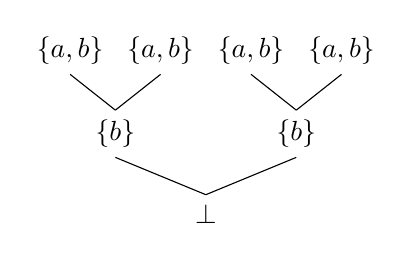
\begin{tikzpicture}[grow'=up]
   \Tree [.$\bot$  [.${\{b\}}$ ${\{a,b\}}$ ${\{\ol a,b\}}$ ] [.${\{ \ol b\}}$ ${\{a, \ol b\}}$ ${\{\ol a, \ol b\}}$ ] ]
   \end{tikzpicture}
   \caption{A resolution tree for Example \ref{exp:res1}.}
   \label{fig:resol1}
   \end{figure}
\end{examp}
%-------------------------------------------------------------------------
\section{DP-reduction}
\label{sec:dpr}

\begin{defi}\label{def:redctn}
A \textbf{reduction} is considered as a map $\bmm{r}: \Cls \ra \Cls$ such that for all $F \in \Cls$, $r(F)$ is satisfiability-equivalent to $F$. Using the reduction technique, unsatisfiability is resulted if $\bot \in r(F)$.
\end{defi}

An example of the reduction is unit resolution (or unit propagation) which is applied to a clause-set $F$ with at least one unit-clause (a clause with one literal). This technique is performed by setting the literal in unit-clause to its satisfying assignment. For example for clause $\set{x}$, consider the literal $x$ to true. If the reduction yields $\bot$, then $F$ is unsatisfiable. Else, if there are more unit-clauses, this step is continued until no unit-clause is left.

\begin{defi}\label{def:dpredc}
By \cite{KullmannZhao2010Extremal}, the \textbf{DP-reduction} is the process of removing a variable $v \in \var(F)$ by taking all clauses having $v$ and replacing them by their resolvents that is:
\begin{displaymath}
\bmm{\dpi{v}(F)} := \set{C \in F : v \notin \var(C)} \cup \set{C \res D : C, D \in F \und C \cap \ol{D} = \set{v}} \in \Cls
\end{displaymath}
\end{defi}
Remarks:
  \begin{enumerate}
  \item If two clauses $C,D \in F$ have more than one clashes, by performing the DP-reduction on one of clashing variables both clauses are removed and we get nothing .
   \end{enumerate}
%%%%%%%%%%%%%%%%%%%%%%%%%%%%%%%%%%%%%%%%%%%%%%%%%%%%%%%%%%
\chapter{Hardness measures for Tseitin graph}
\label{cha:Hd-TseitinG}

\section{Hardness measures}
\label{sec:Hardnessmeasures}

The \textbf{hardness} is defined as a measure of complexity for a representation $F \in \Cls$ of a boolean function $f$ in SAT solving. In this section, two hardness measures are investigated,  the tree-hardness (or just the hardness) and the width-hardness. The first measure is related to the size of resolution proofs while the second one is related to the width of clauses in resolution proofs. We start with defining these measures for unsatisfiable clause-sets and then, we extend the definitions to the satisfiable clause-sets. In Section \ref{sec:game-pd}, a game characterization is given for the tree-hardness and then, in Section \ref{sec:appgame} the game is applied for Tseitin graph.
%-----------------------------------------------------------------------
\subsection{Tree-hardness of clause-sets}
\label{sec:Hardnessunsat}

The unit resolution is explained in Section \ref{sec:dpr}. Another case of the reduction is generalised unit-clause propagation introduced in \cite{Ku99b} and denoted by $\rk_k$. 

\begin{defi}\label{def:rk}
By \cite{Ku99b}, for $F \in \Cls$ the maps $\bmm{\rk_k}: \Cls \ra \Cls$ for $k \in \NNZ$ is called the \textbf{generalised unit-clause propagation} and defined as follows:
  \begin{eqnarray*}
  \rk_0(F) & := &
  \begin{cases}
  \set{\bot} & \text{if } \bot \in F\\ F & \text{otherwise}
  \end{cases}\\
  \rk_{k+1}(F) & := &
  \begin{cases}
  \rk_{k+1}(\pao x1 * F) & \text{if } \ex\, x \in \lit(F) : \rk_k(\pao x0 * F) = \set{\bot}\\ F & \text{otherwise}
  \end{cases}.
  \end{eqnarray*}
This technique removes some forced literals using forced assignments and discovers unsatisfiability if $\bot \in \rk_k(F)$.
\end{defi} 

Remarks:
\begin{enumerate}
  \item For $k=1$, the generalised unit-clause propagation eliminates all unit-clauses with assigning their satisfying assignment. Thus, $\rk_1$ is the \textbf{unit-clause propagation}.
  \item $\rk_2$ is called \textbf{failed literal elimination} and all clauses in $\rk_2$ have length at least $2$ (since all unit-clauses have already been removed).
  \item In each step $k$, if $\rk_k$ yields $\bot$ then the original clause-set $F$ is unsatisfiable while $F$ is satisfiable if $\top$ is obtained. In the latter case, the sequence of forced assignments eliminated until that level is a satisfying assignment for $F$.
  \item $\rk_k(F)$ is computable in time $O(\ell(F) \cdot n(F)^{2(k-1)})$ (by \cite{GwynneKullmann2012Slur}).
  \item The map $\rk_k$ is well-defined since it does not depend on the choices of literals in each step. For example, in the process of obtaining  $\rk_1$ the final result does not change based on the order of choosing the unit literals. 
  \item For all clauses $C \in F$ if $\abs{C} > k$, then $\rk_k(F) = F$. This means that this technique is not complete since $\rk_k(F)$ can not discover the unsatisfiability of a clause-set $F$ if all clauses in $F$ have length at least $k+1$.
\end{enumerate}

\begin{examp}\label{exp:rk}
Using literals $a,b,c,d$, $\rk_k(F)$ for some examples is computed as follows:
  \begin{enumerate}
  \item $\rk_k(\set{\bot}) = \set{\bot}$ for $k \ge 0$ and $\rk_k(\top) = \top$ for $k \ge 0$.
  \item For $F := \set{\set{a},\set{b},\set{c},\set{d}}$: $\rk_0(F) = F$, $\rk_k(F) = \top$ for $k \ge 1$.
  \item For $F := \set{\set{a,b},\set{a,\ol{b}}, \set{\ol{a},b},\set{\ol{a},\ol{b}}}$: $\rk_k(F) = F$ for $k \le 1$, $\rk_k(F) = \set{\bot}$ for $k \ge 2$.
  \end{enumerate}
\end{examp}

One of hardness measures for $F \in \Usat$ is related to the complexity of its resolution proof and reviewed in \cite{GwynneKullmann2013GoodRepresentationsIIex, BeyersdorffKullmann2014PHP,BeyersdorffGwynneKullmann2013PHPER,GwynneKullmann2012Slur}. Following, the Horton-Strahler number is defined as a measure of branching complexity for trees and used for resolution trees $T$.

\begin{defi}\label{def:hsn}
By \cite{BeyersdorffKullmann2014PHP}, the \textbf{Horton-Strahler number} $\bmm{\hts(T)} \in \NNZ$ for each node of a resolution tree $T$ is the length of the shortest path from that node to the leaves. For the root of $T$,  $\hts(T)$ is the height of the tree.
\end{defi}
Remarks:
  \begin{enumerate}
  \item To obtain $\hts(T)$, we start with leaves (axioms) whose Horton-Strahler number are defined as $\hts(T) := 0$. Then, for each inner node with two children $T_1, T_2$, we have two cases. If $\hts(T_1)= \hts(T_2)$, then $\hts(T) := \hts(T_1)+ 1$. Otherwise, $\hts(T) := \max(\hts(T_1),\hts(T_2))$.  For example, for all resolution trees $T:F \vdash \bot$ with $\hts(T) \leq 1$, every node is either a leaf or has a leaf as a child.
\end{enumerate}

\begin{defi}\label{def:hdhs}
Based on \cite{BeyersdorffKullmann2014PHP}, for an unsatisfiable clause-set $F$ there exist a resolution refutation $T:F \vdash \bot$ with the Horton-Strahler number (height) $\hts(T)$. The \textbf{tree-hardness} (or just hardness) for $F \in \Usat$ is defined as the minimum of $\hts(T)$ of all  $T:F \vdash \bot$ and denoted by $\bmm{\hardness(F)} \in \NNZ$.
\end{defi}
Remarks:
\begin{enumerate}
  \item From computational point of view, Definition \ref{def:hdhs} is not a practical method to obtain the hardness. Thus, there is another description using an algorithmic approach via generalised unit-clause propagation $\rk_k$.
  \item According to definition of $\rk_k(F)$ in \ref{def:rk}, the hardness is the minimum of $k \in \NNZ$ such that $\rk_k(F)$ yields $\bot$. This description is extended for satisfiable clause-sets in Definition \ref{def:hd-extended} based on \cite{BeyersdorffKullmann2014PHP, GwynneKullmann2013GoodRepresentationsIIex}.
\end{enumerate}

\begin{lem}\label{lem:hd-phi}
By \cite{GwynneKullmann2012Slur}, for $F \in \Usat$ and every $0 \le k \le \hardness(F)$ there exists a partial assignment $\vp \in \Pass$ such that $n(\vp) = k$ and $\hardness(\vp *F) =\hardness(F) - k$.
\end{lem}

\begin{defi}\label{def:hd-extended}
Based on \cite{BeyersdorffGwynneKullmann2013PHPER}, the hardness is a map that assigns a natural (and finite) number for a representation of a boolean function $f$ as a clause-set $F \in \Cls$ and is denoted by $\bmm{\hardness} : \Cls \rightarrow \NNZ$. To obtain the hardness of  $F$, there are three cases: if $F = \top$, then $\hardness(F) := 0$. Else if $F \in \Usat$, then $\hardness(F) := \min \set{k \in \NNZ : \rk_k(F)=\set{\bot}}$. Otherwise, $F \in \Sat \sm \set{\top}$ and $\hardness(F) := \max \set{ \hardness(\vp * F) : \vp * F \in \Usat }$.
\end{defi}

Remarks:
  \begin{enumerate}
  \item For all full clauses $A_n \in \Usat$, we have $\hardness(A_n)=n$.
  \item By \cite{BeyersdorffGwynneKullmann2013PHPER}, we have $\bmm{\Urefc_k} := \set{F \in \Cls : \hardness(F) \le k}$. The properties of $\Urefc_k$ is investigated in \cite{GwynneKullmann2012Slur}.
  \item For $F \in \Urefc_k$, the decision whether they are satisfiable or not is polynomial time (by \cite{GwynneKullmann2012Slur}).
  \item Every $F \in \Sat \sm \set{\top}$ can be converted to an unsatisfiable clause-set $F' \in \Usat$ by applying a partial assignment $\vp$. 
  \item For extending the hardness measure for $F \in \Sat$ based on Lemma \ref{lem:hd-phi}, we should consider the worst case value of $\hardness$ for $\vp * F \in \Usat$ which is the maximum of $\hardness(\vp * F)$. The reason is that $\hardness(\vp * F) \leq \hardness(F)$ and one can easily find a $\vp$ such that $\bot \in \vp * F$ and $\hardness(\vp * F)=0$. For $\vp$ we only need to consider the minimal partial assignment which is $\vp_C : C \in \primec_0(F)$. For $F = \top$, since it is not convertible to an unsatisfiable clause-set, we assign the minimum of the hardness which is zero.  
  \item $\rk_k$ can not yield $\set{\bot}$ if all clauses in $F$ have length at least $k+1$.
  \item For $F \in \Cls$, in general computing $\hardness(F)$ is not polynomial time. But, there are special groups of clause-sets (as investigated in \cite{GwynneKullmann2012Slur}) that we can compute their hardness in polynomial time. 
\end{enumerate}

\begin{examp}\label{exp:harducls}
For $\set{\set{x,y},\set{x,\ol{y}},\set{\ol{x},y},\set{\ol{x},\ol{y}}}$ we have $r_1(F)=F, r_2(F)=r_2( \langle a \rightarrow 1 \rangle * F) = \{ \bot \}$(since $r_1( \langle a \rightarrow 0 \rangle * F)=r_1 (\{\{ b \}, \{ \ol b \}\}) = \{ \bot \}$). Thus, $\hardness(F) = 2$. In general, the hardness of full clause-sets are as $\hardness(A_n)=n$.
  
Following, $\hardness(F)$ for some more examples of unsatisfiable clause-sets $(F)$ are computed:
  \begin{enumerate}
  \item $\hardness(F) = 0$ if $\bot \in F$.
  \item $\hardness(\set{\set{a},\set{\ol{a}}}) = 1$.
  \item $\hardness(\set{\set{a},\set{\ol{a},b}, \set{\ol{b},c}, \set{\ol{c}}}) = 1$. In general, unsatisfiable Horn clause-sets (whose clauses have at most one positive literal) have hardness one.
  \item $\hardness(\set{\set{a,\ol{b}},\set{\ol{a},b},\set{b,\ol{c}},\set{\ol{b},c},\set{a,b,c},\set{\ol{a},\ol{b},\ol{c}}}) = 2$.
  \end{enumerate}
\end{examp}

\begin{examp}\label{exp:hd-extd}
For $F = \set{\set{x, y} , \set{x,\ol y}} \in \Sat$ with $\primec_0(F) = \set{\set{x}}$,  $\hardness(F)= \max \set{ \hardness(\vp * F) : \vp =\pab{x \ra 0} }=\hardness(\set{\set{y},\set{\ol y}})=1$.
\end{examp}
\begin{lem}\label{lem:hd1}
By \cite{GwynneKullmann2012Slur}, consider $F \in \Cls$ and $v \not \in \var(F)$. If $F' := \set{C \cup \set{v} : C \in F} \cup \set{C \cup \set{\ol{v}} : C \in F}$, Then $\hardness(F') = \hardness(F) + 1$.
\end{lem}
\begin{lem}\label{lem:uck}
Based on \cite{GwynneKullmann2012Slur}, For $F \in \Cls$ and $k \in \NNZ$ we have $F \in \Urefc_k \iff \fa\, C \in \primec_0(F) : F \vdash_k C$ (that is for all prime implicates $C$ of $F$ there is a resolution tree deriving $C$ from $F$ such that there exists a path to some leaf of length at most $k$ from all nodes.
\end{lem}
%-----------------------------------------------------------------
\subsection{Width-hardness of clause-sets}
\label{sec:whdd}

Another measure for the complexity of an unsatisfiable clause-set $F$ as in \cite{BeyersdorffKullmann2014PHP, BeyersdorffGwynneKullmann2013PHPER} is the width-hardness (or asymmetric width) and indicated by $\whardness(F)$. 

\begin{defi}\label{def:kres}
Based on \cite{Kl93}, for a resolution proof $T: F \vdash C$ consider that each node (resolvent) in $T$ have at least one parent with length at most $k$. In this case, the resolvent is called $\bmm{k}$-\textbf{resolvent}. If every resolvent in $T$ is a $k$-resolvent, then $T:F \vdash C$ is called $\bmm{k}$\textbf{-resolution} and denoted by $\bmm{F \vdash^k C}$.
\end{defi}
Remarks:
  \begin{enumerate}
  \item 1-resolution is the unit resolution.
  \item For $k=1,2$, $F \vdash^k \bot$ is decidable in polynomial time while for $k \ge 3$ it is an open question (by \cite{BeyersdorffKullmann2014PHP}).
  %\item Consider $F \in \Usat$. If there exist a $k$-resolution refutation for $F$, then the unsatisfiability can be proved by the unit-preference strategy within $k$ levels (by \cite{Kl93}).
  \item For each $F \in \Usat$ there exist a resolution refutation $T:F \vdash \bot$. The width-hardness of $F$ is the minimum of $k$ for all $k$-resolution trees $T:F \vdash \bot$. This definition is extended for a satisfiable clause-set $F$ in Definition \ref{def:whd-extended} by considering the worst case (maximum) of the width-hardness for the extended $F$ (that is $ \vp * F \in \Usat$) and $\whardness(\top):=0$.
  \end{enumerate}
 
\begin{defi}\label{def:whd-extended}
The \textbf{width-hardness} is a map denoted by $\bmm{\whardness} : \Cls \rightarrow \NNZ$ for a representation of a boolean function $f$ as a clause-set $F \in \Cls$. By \cite{GwynneKullmann2013GoodRepresentations}, to obtain the width-hardness of  $F$ there are three cases: if $F = \top$, then $\whardness(F) := 0$. Else if $F \in \Usat$, then $\whardness(F) := \min \set{k \in \NNZ : F \vdash^k \bot}$. Otherwise, $F \in \Sat \sm \set{\top}$, and $\whardness(F) := \max \set{ \whardness(\vp * F) : \vp * F \in \Usat }$.
\end{defi}

Remarks:
  \begin{enumerate}
  \item By \cite{BeyersdorffKullmann2014PHP}, we have $\bmm{\Wrefc_k}:= \set{F \in \Cls : \whardness(F) \le k}$. 
  \item If $\bot \in F$, then $F \vdash^0 \bot$ and $\whardness(F)=0$. Also if $\rk_1(F)=\set{\bot}$, then it is 1-resolution (unit resolution) and  $\whardness(F)=1$.
  \item For fixed $k \in \NNZ$ and input $F \in \Usat$ the decision whether $\hardness(F) \le k$ or $\whardness(F) \le k$ is solvable in polynomial time (by \cite{BeyersdorffKullmann2014PHP}). 
  \item For $F \in \Usat$, obtaining $\whardness(F) = k$ for $k \in \set{0,1,2}$ is decided in polynomial time, while for $k > 2$ its time complexity is unknown (by \cite{GwynneKullmann2013GoodRepresentationsIIex}).
  \item For $F \in \Usat$, a formula is given to obtain $\whardness(F)$ in \cite{BeyersdorffGwynneKullmann2013PHPER} as follows: if $T$ is a resolution tree for $F$ with $w_1, w_2$ as left and right children and subtrees $T_1, T_2$, then we have:
  \begin{displaymath}
  \whardness(T) := \max \big (\whardness(T_1), \whardness(T_2), \, \min(\abs{C(w_1)}, \abs{C(w_2)}) \big )
  \end{displaymath}
  and $\whardness(F) := \min \set{\whardness(T) \mb T : F \vdash \bot}$.
  \item In \cite{BeyersdorffGwynneKullmann2013PHPER}, another hardness measure is given which is called symmetric width. Also, the relation between this measure and $\whardness$ is discusses in Section 5 of this reference.
  \end{enumerate}
  
\begin{lem}\label{lem:hd-whd}
By \cite{BeyersdorffKullmann2014PHP}, $\Wrefc_0 = \Urefc_0$ and $\Wrefc_1 = \Urefc_1$. Also, for all $F \in \Cls$ we have $\whardness(F) \le \hardness(F)$.
\end{lem}
%-----------------------------------------------------------------
\section{Game characterisations of hardness measures}
\label{sec:game-pd}

In \cite{PI2000}, a game (with two player: Delayer and Prover) is explained to obtain a lower bounds on resolution refutation for $F \in \Usat$. In this game, Delayer starts the game by claiming to know a satisfying assignment for $F$, and Prover wants to expose his lie by asking for a variable value in each round. Then, Delayer can either choose to set some variables to 0/1, or can defer the choice to the Prover. In the latter case, Delayer gets one point. This game is modified to an asymmetric version in \cite{BGL13a} which precisely characterises tree resolution size. In \cite{BeyersdorffKullmann2014PHP,BeyersdorffGwynneKullmann2013PHPER}, the asymmetric version of the game is characterised to obtain $\hardness(F)$ and $\whardness(F)$ of a clause-set $F \in \Cls$. In this game, Delayer starts the game and two players play in turns. There is a partial assignment $\vp \in \Pass: \var(\vp) \sse \var(F)$ (initially empty) that is extended to $\vp'$ by two players. Delayer extend $\vp$ to $\vp'$ such that $\vp' \spe \vp$ while Prover extend $\vp$ to $\vp'$ such that $\vp' \spe \vp$ with $\vp' * F= \top$ or $n(\vp')=n(\vp)+1$. Section \ref{sec:game-hdf} is dedicated to explain the game for obtaining $\hardness(F)$ and in Section \ref{sec:game-whdf} the game for $\whardness(F)$ is presented.

\subsection{Game characterisations of tree-hardness}
\label{sec:game-hdf}

In this section, the modified Prover-Delayer game for obtaining the hardness is discussed. To explain the game, first we need to know that how $\hardness(F)$ for $F \in \Cls$ is changed by assigning a variable in $F$. 

\begin{lem}\label{lem:hd-var}
By \cite{BeyersdorffKullmann2014PHP}, for a clause-set $F \in \Cls$ and $\hardness(F)$ if we assign a value $\ve \in \set{0,1}$ to a variable $v \in \var(F)$, then there are exactly two cases that can happen for $\hardness(F)$. The first case is $\hardness(\pab{v \ra \ve}*F)=\hardness(F)$ and $\hardness(\pab{v \ra \ol \ve}*F) \leq \hardness(F)$ and the second case is  $\hardness(\pab{v \ra \ve}*F)=\hardness(\pab{v \ra \ol \ve}*F)=\hardness(F)-1$. Thus, for all cases  $\hardness(\pab{v \ra \ve}*F) \leq \hardness(F)$.
\end{lem}

\begin{defi}\label{def:var-trb}
For $F \in \Cls$ and  $\ve \in \set{0,1}$, a variable $v \in \var(F)$ is called \textbf{trouble maker} if $\hardness(\pab{v \ra \ve}*F)=\hardness(F)$ and $\hardness(F)- \hardness(\pab{v \ra \ol \ve}*F) \geq 2$. Also, if $\hardness(\pab{v \ra \ve}*F)=\hardness(\pab{v \ra \ol \ve}*F = \hardness(F)$ then $v$ is called \textbf{ineffective variable}.
\end{defi}

Based on \cite{BeyersdorffKullmann2014PHP}, the strategy of Delayer is to maximize the points he gets (to maximize $\hardness(F)$ for $F \in \Cls$) while Prover wants to minimize the points that Delayer gets (to minimize the hardness of $F$). Also, \cite{BeyersdorffKullmann2014PHP} considers a global partial assignment $\vp \in \Pass$ which is extended to $\vp' \spe \vp$ in each round. Here, the extension of the partial assignment is considered as a sequence in Definition \ref{def:atomicm}.

\begin{defi}\label{def:atomicm}
For $F \in \Cls$, there is a sequence of partial assignments $\vp_0, ..., \vp_m \in \Pass$ for Prover-Delayer game ($m \in \NN$ is the number of rounds played in the game) such that $\vp_0=\epa$ and $\vp_i \spe \vp_{i-1}$ with $1 \le i \le m$ and $\var(\vp_i) \sse \var(F)$. The \textbf{atomic move} of the Prover-Delayer game introduced in \cite{BeyersdorffKullmann2014PHP} can be defined as the extension of the partial assignment $\vp_{i-1} $ to $\vp_{i}$ by each player and in the case of Prover, also holds $n(\vp_i)=n( \vp_{i-1})+1$.
\end{defi}

\begin{lem}\label{lem:atm-m-D-P}
In the case of Prover-Delayer game for obtaining the hardness of $F \in \Cls$, the \textbf{optimal atomic move} for Delayer is removing all trouble makers in Definition \ref{def:var-trb} by assigning them such that $\hardness(\pab{v \ra \ve}*F)=\hardness(F)$ (the hardness remains unchanged). If htere is no trouble maker, Delayer defers the assignment to Prover. For Prover, the atomic move is assigning exactly one variable $v \in \var(F)$ such that the hardness decreases exactly one unit.
\end{lem}
\begin{prf}
The aim of Delayer is to maximize $\hardness(F)$ for $F \in \Cls$. But since according to Lemma \ref{lem:hd-var} assigning a variable for $F$ does not increase the hardness, Delayer must keep $\hardness(F)$ unchanged. This is achieved by taking no action or just assigning  ineffective variables. On the other hand, Prover wants to minimize $\hardness(F)$ and in each round, tries to choose a variable $v \in \var(F)$ whose assigning reduces the hardness at most (like two or more units). Thus, Delayer must prevent the case that Prover decreases the hardness more than one unit. This is achieves by assigning the trouble makers such that $\hardness(F)$ remains unchanged. If Delayer succeeds in removing all trouble makers in each round, then Prover must decrease $\hardness(F)$ exactly one unit.
\end{prf}

In \cite{BeyersdorffKullmann2014PHP}, the game for obtaining the hardness of $F \in \Cls$ is explained as performing an atomic move (as the extension of the global assignment $\vp$) and the game ends once $\bot \in \vp * F $ or $\vp * F=\top$ is reached. Here, the game is re-defined using Definition \ref{def:atomicm} for the sequence of partial assignments and Lemma \ref{lem:atm-m-D-P} for atomic move.

\begin{lem}\label{lem:hd-game-main}
Consider $F \in \Cls$. The Prover-Delayer game to obtain $\hardness(F)$ is as follows:
  \begin{enumerate}
  \item Delayer starts the game and two players play in turns.
  \item Both players perform one optimal atomic move (defined in Lemma \ref{lem:atm-m-D-P}) in each round.
  \item Considering $\vp_m$ in Definition \ref{def:atomicm}, the game ends once $\bot \in \vp_m * F $ (if $F$ is unsatisfiable) or $\vp_m * F=\top$ (if $F$ is satisfiable) is reached. 
  \end{enumerate}
\end{lem}
Remarks:
  \begin{enumerate}
  \item The game has a finite number of rounds $m \in \NN$ since there is a finite number of variables in clause-sets $F \in \Cls$. 
  \end{enumerate}

\begin{lem}\label{lem:hdchg}
Consider the game in Lemma \ref{lem:hd-game-main} for $F \in \Cls$ with $m \in  \NN$ rounds ($m$ is finite) and $\vp_i \in \Pass$ in Definition \ref{def:atomicm}. If $F_i:= \vp_i * F$ with $1 \le i \le m$, we have:
  \begin{eqnarray*}
  \hardness(F_i) & = &
  \begin{cases}
  \hardness(F_{i-1}) & \text{Delayer's turn }\\ \hardness(F_{i-1})-1 & \text{Prover's turn}
  \end{cases}
  \end{eqnarray*}
Also, $\hardness(F_m)=0$.
\end{lem}
\begin{prf}
By Lemma \ref{lem:atm-m-D-P} and \ref{lem:hd-game-main}.
\end{prf}

\begin{lem}\label{lem:gameres1}
Consider the Prover-Delayer game in Lemma \ref{lem:hd-game-main} for $F \in \Cls$. The hardness $\hardness(F)$ is exactly the number of rounds played by Prover (or we can say that Prover gets a point in by performing an atomic move and the hardness of $F$ is equal to Prover's points).
\end{lem}
\begin{prf}
For $F \in \Cls$, based on Lemma \ref{lem:hdchg} if the game is played in $m$ rounds, then $\hardness(F_m)=0$ . Also, in each round played by Prover the $\hardness(F)$ is decreased exactly by one unit and in the other rounds, it remains unchanged. Therefore, $\hardness(F)$ is the number of rounds played by Prover.
\end{prf}
Remarks:
  \begin{enumerate}
  \item It should be mentioned that by considering performing exactly one atomic move in each round, the number of rounds $m$ is an even number. Thus, saying that the hardness equals to $m / 2$ is equivalent to the above statement.
  \end{enumerate}
  
\begin{quest}\label{que:game-move}
In Definition \ref{lem:atm-m-D-P}, the atomic move for Delayer is defined as removing trouble makers. If Delayer removes one or more ineffective variable, does the game still obtain $\hardness(F)$ for $F \in \Cls$?
\end{quest}
%------------------------------
\subsection{Game characterisations of width-hardness}
\label{sec:game-whdf}

In \cite{BeyersdorffKullmann2014PHP}, a modified version of Prover-Delayer game is given to obtain the width-hardness of only unsatisfiable clause-sets. In this game, strategy of Delayer is to maximize $\whardness(F)$ while the strategy of Prover is to minimize $\whardness(F)$. There is a global partial  assignment $\vp \in \Pass$ with $\var(\vp) \sse \var(F)$ and initially empty which is extended by players and the game ends one $\bot \in \vp * F$ is achieved.

\begin{lem}\label{lem:whdgame}
By \cite{BeyersdorffKullmann2014PHP}, for $F \in \Usat$ the Prover-Delayer game to obtain $\whardness(F)$ is as follows:

  \begin{enumerate}
  \item The two players play in turns, and Delayer starts.
  \item Delayer extends $\vp$ to $\vp' \supseteq \vp$.
  \item Prover chooses some $\vp'$ compatible with $\theta$ such that $\abs{\var(\vp') \sm \var(\vp)} = 1$.
  \item If $\bot \in \vp * F$, then the game ends, and Delayer gets the maximum of $n(\vp')$ chosen by Prover as points ($0$ if Prover didn't make a choice).
  \item Prover plays in such a way that the rounds of game is finite.
  \end{enumerate}
  \end{lem}
Remarks:
  \begin{enumerate}
  \item According to \cite{BeyersdorffKullmann2014PHP}:
  \begin{enumerate}
  \item In this game, Delayer achieves $k \in \NN$ points whatever Prover does and wants to achieve $\whardness(F) \ge k$. Since the strategy of Delayer is to maximize the points he gets, thus it guarantees to obtain at least $\whardness(F)$ many points.
  \item Prover guarantees that Delayer gets at most $k \in \NNZ$ points in any case and wants to achieve $\whardness(F) \le k$. Since the strategy of Prover is to minimize points, Thus it guarantees to obtain at most $\whardness(F)$ many points for Delayer (whatever Delayer does).
  \end{enumerate}
  \end{enumerate}

\begin{quest}\label{que:whdall}
Can we generalise the game characterisation of width-hardness for all clause-sets  $F \in \Cls$?
\end{quest}
%%%%%%%%%%%%%%%%%%%%%%%%%%%%%%%%%%%%%%%%%%%%%%%%%%%%%%%%%%
\section{XOR representation}
\label{sec:XOR representation}

The CNF-clause-sets is defined in Section \ref{sec:Clause-sets}. In this section, XOR-clause-set is explained for extending the hardness game for graphs. An XOR-clause-set for $f$ is the interpretation of a clause-set $F \in \Cls$ as a system of XOR-constraints whose clauses $C$ are parity equation for $v \in \var(C)$. This representation is investigated in \cite{GwynneKullmann2013GoodRepresentations,GwynneKullmann2013GoodRepresentationsIIex,GwynneKullmann2013GoodRepresentationsIILata} with the goal of finding a good representation for XOR-constraints.

\begin{defi}\label{def:xor-const} 
An \textbf{XOR-constraint} (or parity constraint) is a boolean function (parity function) $f$ in the form of $x_1 \oplus \dots \oplus x_n = \ve$ that $x_1, \dots, x_n \in \Lit$ and $\ve \in \set{0,1}$.
\end{defi}

Remarks:
\begin{enumerate}
    \item $x_1 \oplus \dots \oplus x_n = y$ is equivalent to $x_1 \oplus \dots \oplus x_n \oplus y = 0$
    \item $x \oplus x = 0$, $x \oplus \ol{x} = 1$, $0 \oplus x = x$, $1 \oplus x = \ol{x}$.
    \item Two XOR-constraints $f_1, f_2$ are equivalent iff $\var(f_1) = \var(f_2)$ and both have the same parity for literals.
\end{enumerate}

\begin{defi}\label{def:xor-cls}
Based on \cite{GwynneKullmann2013GoodRepresentationsIIex}, an \textbf{XOR-clause} $C \in \Cl$ with literal $x \in \Lit$ is an XOR-constraint with $\oplus_{x \in C} = 0$. Thus, two XOR-clauses $C, D$ are equivalent iff $\var(C) = \var(D)$ and both with the same parity. In an XOR-clause, there is no repetitive literals since $x \oplus x = 0$. In the case of clashing literals, we remove them using the laws $x \oplus \ol{x} = 1$ and $1 \oplus y = \ol{y}$ (since according to the definition, clashing literals are not allowed in clauses).

An \textbf{XOR-clause-set} is a clause-set $F \in \Cls$ whose clauses $C$ are interpreted as an XOR-clause.  
\end{defi} 

Remarks:
\begin{enumerate}
  \item The operation of a partial assignment $\vp \in \Pass$ to XOR-clause-sets is defined as the same definition for CNF-clause-sets.
  \item An XOR-clause-set $F$ is satisfiable if there exist a partial assignment $\vp$ such that $\var(\vp) \supseteq \var(F)$ and for every $C \in F$ the number of $x \in C$ with $\vp(x) = 1$ is even (that satisfies the equation  $\oplus_{x \in C} = 0$).
\end{enumerate}

The satisfiability of a CNF-clause-set is investigated using the resolution operation. Here, for investigating whether an XOR-clause-set is satisfiable or not, an operation is defined based on \cite{GwynneKullmann2013GoodRepresentationsIIex,GwynneKullmann2013GoodRepresentationsIILata} which is called an XOR-sum over clauses of $F$.

\begin{defi}\label{def:xor-sum}
By \cite{GwynneKullmann2013GoodRepresentationsIIex}, the \textbf{XOR-sum} over clauses of $F$ denoted by $\oplus F \in \Cl$ is applied to two XOR-clauses and produces a new clause or the result is inconsistent. The operation is performed as follows. If there are four literals as $x,\ol{x},y,\ol{y}$ for $x \ne y$, the XOR-sum of them is as $x \oplus \ol{x} = 1$ and $y \oplus \ol{y} = 1$. Thus, $1 \oplus 1 = 0$ and they are removed. If no clash remains, then the result is obtained as a clause $E \in \Cl$. Else if there is just one clash for literals $x, \ol{x}$ with at least one other literal $y$, then $x \oplus \ol{x} = 1$ and $1 \oplus y=\ol{y}$ and a new clause $E \in \Cl$ is obtained. Otherwise, if two literals $x, \ol{x}$ remains, then $\oplus F$ is called inconsistent. 

An XOR-clause-set $F \in \Cls$ is unsatisfiable if and only if there is $F' \sse F$ such that $\oplus F'$ is inconsistent.
\end{defi} 

\begin{examp}\label{exp:xorcls}
The satisfiability of the following XOR-clause-sets $F$ are investigated using the XOR-sum over clauses of $F$.
  \begin{enumerate}
  \item For $F=\top$, $ \oplus(F)= \oplus(\set{\bot})=\bot$ and $F$ is satisfiable.
  \item For $F=\set{\set{a,b},\set{b,c,\ol d}}$, $ \oplus(F) = \set{a,c,\ol d}$ and $F$ is satisfiable.
  \item For $F=\set{\set{a,b,c},\set{a, \ol b, \ol c}}$, $ \oplus(F) = \bot$ and $F$ is satisfiable.  
  \item  For $F=\set{\set{a,b},\set{a, \ol b},\set{c,d}}$, $\oplus (F)$ is inconsistent and $F$ is unsatisfiable.
  \end{enumerate}
\end{examp}

For each XOR-clause-set $F$ there is a unique equivalent CNF-clause-set $F'$ (without auxiliary variables). To obtain this equivalent CNF-clause-set, a translation is defined and indicated by $X_0(F)$. This translation, converts each clause of $F$ to a set of full clauses in CNF-representation and then $F'$ is the union of these sets. If $F$ has long clauses, then obtaining $X_0(F)$ is not practical.

\begin{defi}\label{def:x0tr}
By \cite{GwynneKullmann2013GoodRepresentationsIIex}, the \textbf{$X_0$ translation} is a map $X_0: \Cls \ra \Cls$ where the input is an XOR-clause-set and the output is a  CNF-clause-set. Consider an XOR-clause $C \in F$, the $X_0$ translation of this clause is defined as the set of prime implicates of the boolean function for $C$ (without auxiliary variables) and indicated by $X_0(C)=\primec_0(x_1 \oplus \dots \oplus x_n = 0)$. The translation $X_0(C)$ contains all the full clauses over the set of variables in $C$ whose parity are different from the parity of $C$. Thus, $\abs{X_0(C)}=2^{\var(C)-1}$. Finally, the CNF-clause-set is obtained by $X_0(F) := \bc_{C \in F} X_0(C)$.
\end{defi} 

\begin{examp}\label{exp:X0}
For $F=\set{\set{a,\ol b}}$, $X_0(F)= \set{\set{a,b},\set{\ol a,\ol b}}$ and for $F=\set{\set{a},\set{b,c}}$, $X_0(F)=\set{\set{\ol a},\set{\ol a, b}, \set{a, \ol b}}$.
\end{examp}
%-----------------------------------------------------------------
\subsection{Tseitin graph}
\label{sec:Tseitin graph}

For extending the hardness game for graphs, first we need to describe Tseitin graph and Tseitin clause-set. 
\begin{defi}\label{def:graph}
Based on \cite{GwynneKullmann2013GoodRepresentationsIIex}, a simple graph is a pair $G = (V,E)$ where $V$ is the set of vertices and $E$ is the set of edges. If the graph is considered as a triple $\bmm{G = (V,E,\eta)}$ such that $V$ is the set of vertices, $E$ is the set of edge-labels and $\eta: E \ra \set{e \sse V : 1 \le \abs{e} \le 2}$, then parallel edges and loops can be described. 
\end{defi}
Remarks:
  \begin{enumerate}
  \item Consider a connected graph $G=(V,E,\eta)$ without loop. First, we label each edge with a distinct literal $x \in E$. Then, if we assign a \textbf{charge} $\bmm{\rho}$ to each vertex such that $\rho: V \ra \set{0,1}$, a unique XOR-clause-set corresponded to $G$ is obtained. In this case, each vertex $w \in V$ is specified as an XOR-clause $C \in \Cl$ such that $\bmm{\oplus_{x \in E, w \in \eta(x)} \; x = \rho(w)}$. Then, the XOR-clause-set for $G$ is obtained by $T_0(G,\rho) := \set{C_w : w \in V} \in \Cls$. 
  \end{enumerate}

\begin{lem}\label{lem:chgvar}
 For a graph $G=(V,E,\eta)$ without loop, consider $T_0(G,\rho)$ an XOR-clause-set. Based on \cite{Ts68} Section 2, we define $\Phi$ as an XOR-constraint for charges of vertices that is $\oplus_{w \in V} \rho(w) = \ve$ and $\ve \in \set{0,1}$. By assigning a value to all edges $x \in E$, we obtain $\rho(w)$ of all vertices and then, the value of $\ve$ in $\Phi$. In this case, if we change the value of an edge $x$, then $\rho(w)$ for each endpoint of $x$ must be changed to keep $\Phi$ unchanged.
\end{lem}
\begin{prf}
According to the definition, each vertex $w$ of $G$ is an XOR-clause with $\rho(w)$ such that  $\oplus_{x \in E, w \in \eta(x)} \; x = \rho(w)$ ($\rho$ is the parity). Since each literal corresponds to an edge connected to two vertices $w_1, w_2$, changing the value of a literal $x$ will change the parity $\rho(w)$ for equations of $w_1, w_2$. Thus, by changing the value of an edge, these two equation must be changed to $\Phi$ remains unchanged.
\end{prf}
Remarks:
  \begin{enumerate}
  \item For a graph as in Lemma \ref{lem:chgvar} with $\Phi$, if $\ve=0$ then we need to investigate the satisfiability of each XOR-clause to determine whether $T_0(G,\rho)$ is satisfiable or not. Else if $\ve=1$, then $T_0(G,\rho)$ is unsatisfiable. The reason is as follows. If $\ve=1$ in $\Phi$, there is at least one vertex $w$ (XOR-clause $C$) with $ \rho(w) =1$ and according to the definitions in Section \ref{sec:XOR representation}, an XOR-clause $C$ is satisfiable if $\oplus_{x \in C} = 0$. Thus, $\oplus_{x \in C} = \rho(w) \not =0$ and $T_0(G,\rho)$ is unsatisfiable.
  \end{enumerate}

\begin{defi}\label{def:tseitindef}
By \cite{GwynneKullmann2013GoodRepresentationsIIex}, a graph $G$ as explained in Lemma \ref{lem:chgvar} with $\ve=1$ in $\Phi$, is called a \textbf{Tseitin graph}. The equivalent CNF-clause-set of $G$ is obtained by $X_0$ translation of $T_0(G,\rho)$ and indicated by $\bmm{T(G,\rho)} := X_0(T_0(G,\rho))$. The clause-set $T(G,\rho) \in \Usat$ is called the \textbf{Tseitin clause-set} of $G$.
\end{defi}
Remarks:
  \begin{enumerate}
  \item The clause-set $T(G,\rho) \in \Usat$ is an special subset of clause-sets $F \in \Usat$ and all variables $v \in \var(T(G,\rho) )$ are occurred at most in two clauses (every edge is labeled with a distinct variable). In the case of hypergraph (as in \cite{BeyersdorffGwynneKullmann2013PHPER}), we have hyperedges and variables occurring in more than two clauses are allowed.
  \item Removing an edge $e \in E$ from a Tseitin graph $G$ is equivalent to assigning a value to $e$.
\end{enumerate}
%----------------------------------------------
\section{Application of game characterisation for Tseitin graph}
\label{sec:appgame}

In Section \ref{sec:game-hdf}, a game is explained to obtain the hardness of a clause-set $F \in \Cls$. In this section, This game is applied to a Tseitin graph (with Tseitin clause-set $T(G,\rho) \in \Usat$). %For this reason, first the concept of atomic move is explained for Tsitin graph. Then, the structure of a tree (game-tree) showing all possible atomic moves for a Tseitin graph is given. Finally, the game is applied for a Tseitin graph. 

%In this section based on the game characterisation of the hardness in Section \ref{sec:game-hdf}, a game is explained to obtain the hardness of a Tseitin graph (with Tseitin clause-set $T(G,\rho) \in \Usat$). For this reason, first the concept of atomic move is explained for Tsitin graph. Then, the structure of a tree (game-tree) showing all possible atomic moves for a Tseitin graph is given. Finally, the game is applied for a Tseitin graph.
 
\begin{defi}\label{def:bridge}
Consider a Tseitin graph $G$ as explained in Section \ref{sec:Tseitin graph}. If there is an edge $e \in E$ whose deletion increases the number of connected components of $G$, then $e$ is called a \textbf{bridge}.
\end{defi} 

\begin{lem}\label{lem:game3}
In a Tseitin graph $G$ if an edge $e \in E$ is removed, then $\rho(w)$ of both endpoints will be changed to keep $G$ unsatisfiable. 
\end{lem}
\begin{prf}
According to the Definition \ref{def:tseitindef} of a Tseitin graph $G$, the XOR-clause-set $T_0(G,\rho)$ is unsatisfiable since $\ve=1$ for $\Phi$. Thus, based on Lemma \ref{lem:chgvar} by removing any edge (assigning a value to a variable) the equation of endpoints must be changed to keep $\ve=1$ unchanged.
\end{prf}
Remarks:
  \begin{enumerate}
  \item For a Tseitin graph $G$, removing a bridge (assigning a variable) divides $G$ into two components $G_1,G_2 $ with $T(G_1,\rho), T(G_2,\rho) \in \Usat$. If the hardness of $G$ is indicated by $\hardness(T(G,\rho))$, then we have $\hardness(T(G_1,\rho)), \hardness(T(G_2,\rho)) \le \hardness(T(G,\rho)) $ (by Lemma \ref{lem:hd-var}). In this proposal  report,  $\hardness(T(G_1,\rho)), \hardness(T(G_2,\rho))$ are indicated by  $\hardness_1$ and $\hardness_2$ respectively.
\end{enumerate}

Consider the game in Lemma \ref{lem:hd-game-main} for obtaining the hardness of $F \in \Cls$. The game is performed between two players by removing some variables (assigning some variables) in each round. In \cite{BeyersdorffKullmann2014PHP}, this game is applied for a Tseitin graph $G$ to obtain the hardness of $T(G,\rho)$ as follows:

%In the case of Delayer, based on \cite{BeyersdorffKullmann2014PHP} the atomic move is just removing some variables while in the case of Prover, it is removing exactly one variables. Now for a Tseitin graph, based on this expression of atomic move (and also by considering removing at most one variable in each round), there is a tree (as in Lemma \ref{lem:game-tree}) showing all possible moves for the two players. The hardness of the graph $G$ can be obtained using this tree. Then, the atomic move is optimized for a Tsetin graph in Lemma \ref{lem:atmv} to apply this game for a this graph.


\begin{lem}\label{lem:game-tseitin-hd}
By \cite{BeyersdorffKullmann2014PHP}, consider  $G$ as a non-trivial Tseitin graph. Then $\hardness(T(G,\rho))$ is characterised by the following game:
  \begin{enumerate}
  \item An atomic move for $G$ is defined as removing some $e \in E(G)$ and choosing a connected component of $G - e$. 
  \item The two players play in turns, and Delayer starts with $G$.
  \item A move of Delayer is to apply a sequence of atomic moves (possibly zero).
  \item A move of Prover is to apply exactly one atomic move.
  \item The games ends when $G$ becomes trivial, in which case Delayer gets as many points as there have been moves by Prover (which is equal $\hardness(T(G,\rho))$).
  \end{enumerate}
\end{lem}

\begin{lem}\label{lem:game-tree}
Consider the game in Lemma \ref{lem:game-tseitin-hd} for a Tseitin graph $G$ with the Tseitin clause-set $T(G,\rho) \in \Usat$. For every $G$, there exist a unique tree called \textbf{game-tree} such that shows all possible moves for Prover and Delayer (as removing at most one $e \in E(G)$ and choosing the connected component $G-e$). The tree is upside down with even number of levels (the number of game's rounds is always even) and the root of the tree labeled by $F$. Each level shows the possible moves for a player. Also, every node of the game-tree (except leaves) corresponds to a clause-set $T'(G,\rho)$ ($ \bot \not \in T'(G,\rho)'$) such that the difference between the number of variables in $F'$ and the upper-level nodes is at most one. The children of each node are the all possible atomic moves in that round. It should be mentioned that if Prover can finish the game in one move, then it would do that. Each path from root must end in a leaf since the edges of graph (which correspond to the maximum of atomic moves of Prover) are finite and the leaves correspond to $\bot$. The hardness of $F$ is achieved by assigning a number to each node (starting from leaves) and obtaining the number of the root based on the strategy of Delayer (maximizing points) and Prover (minimizing points).
%Consider a Tseitin graph $G$ of the Tseitin clause-set $T(G,\rho) \in \Usat$ as in Section \ref{sec:Tseitin graph}. Based on Lemma \ref{lem:game-tseitin-hd}, for every $G$, there exist
\end{lem}
\begin{prf}
To obtain the harness, first we assign a number to each leaf that corresponds to the scores of Prover (the number of Prover's atomic moves) through the path to that leaf. Since the last round of game is always played by Prover, we assign the minimum number of leaves to their parents (upper-level nodes). Then, we consider the upper level which is played by Delayer and therefore, we assign the maximum number of nodes for their parents. This process is continued until we get the root and and we assign the maximum number of root's children to the root (since the first round is played by delayer). Finally, the hardness of $F$ corresponds to the number assigned to the root.
\end{prf}
Remarks:
  \begin{enumerate}
  \item The hardness game has finitely many moves since the edges of a Tseitin graph are variables of a clause-set $T(G,\rho) \in \Usat$ (and the number of variables in a clause-set is finite). 
  \item The game is well-defined since it does not depend on choices.
  \end{enumerate}
  
\begin{examp}\label{exp:gg1}
Fig \ref{fig:gg1} shows the game-tree for graph $K_3$ (complete graph with 3 vertices). The children of each node are all possible moves (whether the move is optimal or not) in hardness game for $K_3$. Here, $\ve $ shows the empty move (or when delayer decides to remove no edge) and $\bot$ shows the end of game. The game starts from leaves by counting the number of prover's moves until that leaf and assign this number to that leaf. Then, by considering the maximum assigned number in the Delayer's level and the minimum number in the Prover's level we get the $\hardness(K_3)=2$.
   \begin{figure}
   \begin{center}
   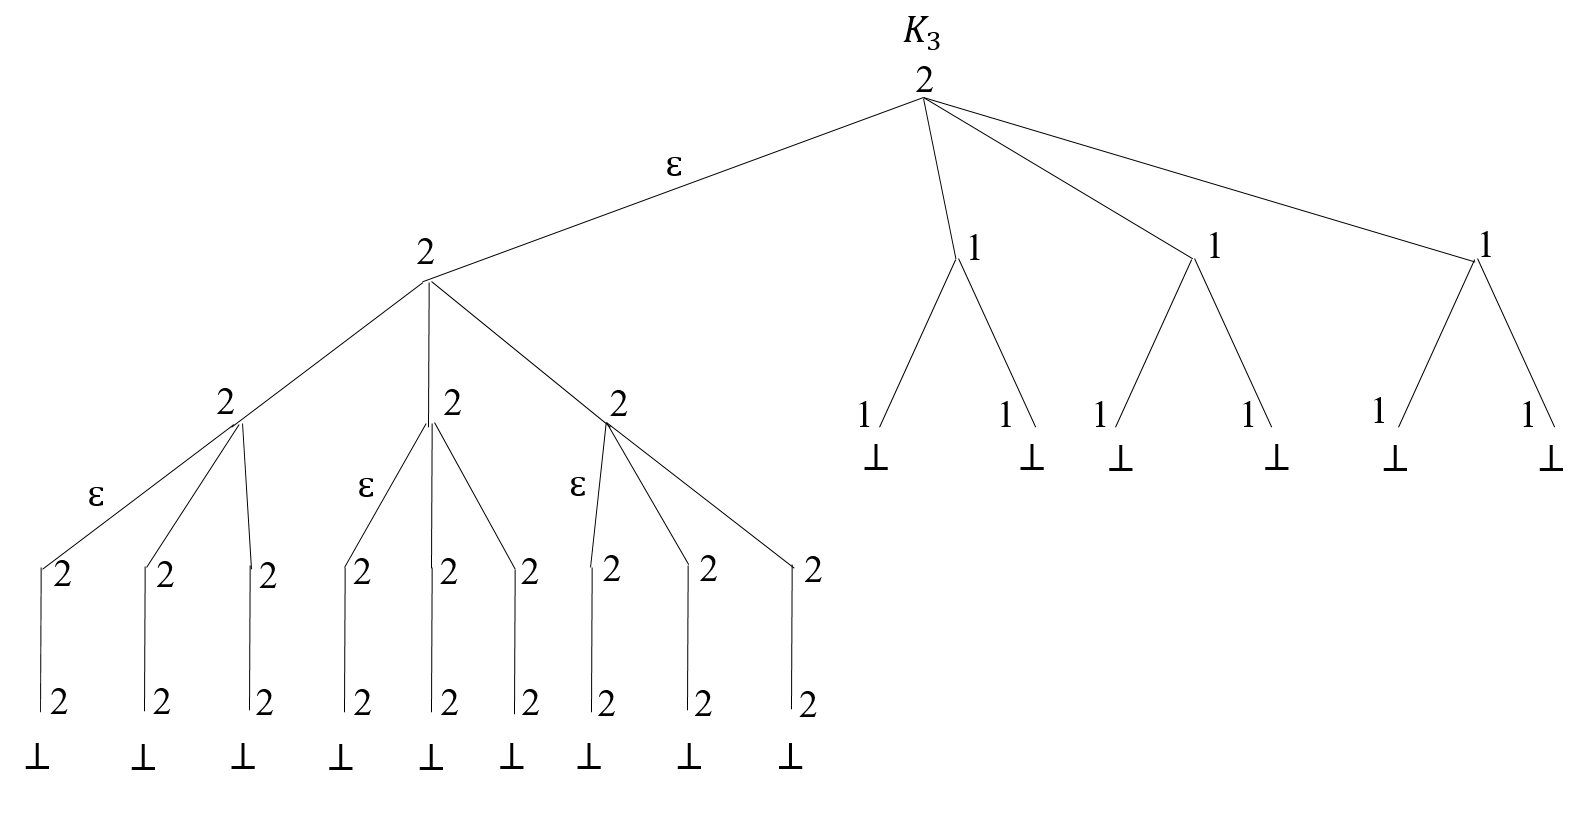
\includegraphics[scale =0.45]{gg1.png}
   \caption{The game-tree for $K_3$.}
   \label{fig:gg1}
   \end{center}
   \end{figure}
\end{examp}
%The optimal value for the hardness of a Tseitin graph $G$ would be in the case that both players play optimally. The optimal move for Delayer is the one which maximizes the hardness and for Prover, the move that minimizes the hardness. Based on Lemma \ref{lem:game-tree}, the optimal move is explained as atomic move in Lemma \ref{def:atmv}.

\begin{lem}\label{lem:tseitin-game-bridge}
Consider a Tseitin graph $G \not = K_2$ with a bridge $e \in E$ such that connects two components $G_1,G_2$ with $\hardness_1$ and $\hardness_2$. In the case of Delayer, the optimal atomic move is to remove the edge and discard the component with smaller hardness (that is having less edges) and the game is continued with the other component. In the case of Prover, the optimal atomic move is to remove the bridge and discard the component with bigger hardness.
\end{lem}
\begin{prf}
Based on Section \ref{sec:game-pd}, the strategy of Delayer is to delay the game while for the Prover it is vise verse. If $G=K_2$, then Delayer must not remove the bridge otherwise the game ends. Else if $G \not = K_2$, then Delayer should remove the bridge and choose the component with bigger hardness to delay the game (to prevent the case that Prover chooses the smaller component). Otherwise Prover removes the bridge and chooses the smaller component to finish the game ASAP.
\end{prf}

\begin{lem}\label{lem:hd1hd2}
Consider a Tseitin graph $G \not = K_2$. If there is a bridge $e \in E$ such that connects two components $G_1,G_2$ with $\hardness_1$ and $\hardness_2$, then there are two cases for $\hardness_{total}$. If $\hardness_1= \hardness_2$, then $\hardness_{total}= \hardness_1= \hardness_2$. Else, $ \abs {\hardness_1- \hardness_2 } \geq 1$ and if $ \hardness_1 > \hardness_2 $  then $\hardness_{total}= \hardness_1$.
\end{lem}	
\begin{prf}
Based on Lemma \ref{lem:game-tseitin-hd}, Delayer starts the game. If $\hardness_1= \hardness_2$, then it does not change the result whether Delayer removes the bridge or it chooses to do nothing and Prover removes the bridge in next move. In both cases $\hardness_{total}$ would be equal to the hardness of the selected component. Otherwise, if $ \hardness_1 > \hardness_2 $ based on \ref{lem:tseitin-game-bridge} Delayer removes the bridge and discards the  component with smaller hardness. In this case, Prover has not performed any move and it did not get any points. Thus, in the next step Prover continues the game and  $\hardness_{total}= \hardness_1$.
\end{prf}

\begin{lem}\label{lem:troubllemk-hd}
Consider a Tseitin graph $G$. The trouble maker variables is Definition \ref{def:var-trb} for $G$ are bridges.
\end{lem}
\begin{prf}
Consider Lemma \ref{lem:hd1hd2}. If $ \abs {\hardness_1- \hardness_2 } \geq 2$ and Delayer does not remove the bridge, then Prover can remove the bridge and get more than one points. Thus, this situation must be prevented by Delayer. This is equivalent to the Definition\ref{def:var-trb} for trouble makers.
\end{prf}

\begin{lem}\label{lem:atmvtseitin}
Consider the game in Lemma \ref{lem:game-tseitin-hd} for a Tseitin graph $G$ with Tseitin clause-set $T(G,\rho) \in \Usat$. The optimal atomic move in Lemma \ref{lem:atm-m-D-P} for this game is as follows:
  \begin{enumerate}
  \item In the case of Delayer, if $G \not = K_2$, the optimal atomic move is removing all bridges (trouble makers) and then choosing the component with the biggest hardness (and discarding other components). 
  \item In the case of Prover, there are two possible situations. If there is no bridge in the graph then the optimal atomic move for Prover is not clear but it should remove an edge. If there is only one bridge, then the optimal atomic move is removing the bridge and choosing the component with the smallest hardness (and discarding other components). In both cases, the hardness decreases one unit.
  \end{enumerate}
\end{lem}
\begin{prf}
Based on Lemma \ref{lem:tseitin-game-bridge} and \ref{lem:troubllemk-hd}.
%Section \ref{sec:game-hdf}, we know that Delayer wants to maximize the hardness (delay the game) while Prover wants to minimize it (finishing the game ASAP). Suppose that there is a bridge $e \in E$ in $G$ which divides it into two components $G_1,G_2$ with $\hardness(T(G_1,\rho)), \hardness(T(G_2,\rho))$. If Delayer does not remove $e$, then Player can remove this bridge by assigning troble makers such than ????and choose the smaller component. In this case, $\hardness(T(G,\rho))$ may go down more than one unit and Prover gets more than one point. Thus, Delayer must prevent this situation by removing all bridges
\end{prf}
Remarks:
  \begin{enumerate}
  \item We are not interested in Prover plays optimally if Delayer has already made a mistake.
  \item If Prover can get two or more points by one move, then Delayer has made a mistake before.
  \end{enumerate}

%\begin{lem}\label{lem:Tseitingame1}
%The game with optimal atomic move is well-defined (it does not depend on choices). 
%\end{lem}
%\begin{prf}
%According to Lemma \ref{lem:atmvtseitin}, in each round Delayer removes all edges that are bridge (trouble maker) to prevent the case that the hardness reduction is more than one unit. Thus, the result of the game does not depend to the order of choosing edges in each round.
%\end{prf}

\begin{examp}\label{exp:hd-K3}
Fig \ref{fig:game1} shows the Prover-Delayer game based on optimal atomic move in Lemma \ref{lem:atmvtseitin} for graph $K_3$ in Fig \ref{fig:hd1}. In this game, Delayer starts the game and since the graph has no bridge, Delayer differs the choice to Prover. Then, Prover removes an edge (in this case, he can remove any edge). In third move, Delayer has to do nothing since removing any edge will lead to ending the game. Thus, Prover removes an edge and the graph is divided to two components: one isolated vertex and one edge. Prover chooses the vertex (the smaller component) to finish the game. The hardness of the graph (which is the number of moves done by Prover) is as $\hardness(K_3)=2$.
  \begin{figure}%[h]
  \centering
  \begin{tabular}{|c|c|} 
                  \hline
                  Delayer & Prover \\ \hline
                  empty move & removing edge 1  \\ \hline
                  empty move & removing edge 3 and keeping the smaller component \\ \hline
  \end{tabular}
  \caption{The optimal atomic moves for graph $K_3$ in Fig \ref{fig:hd1} with $\hardness(K_3)=2$.}  \label{fig:game1}
  \end{figure}
  \begin{figure}
  \begin{center}
  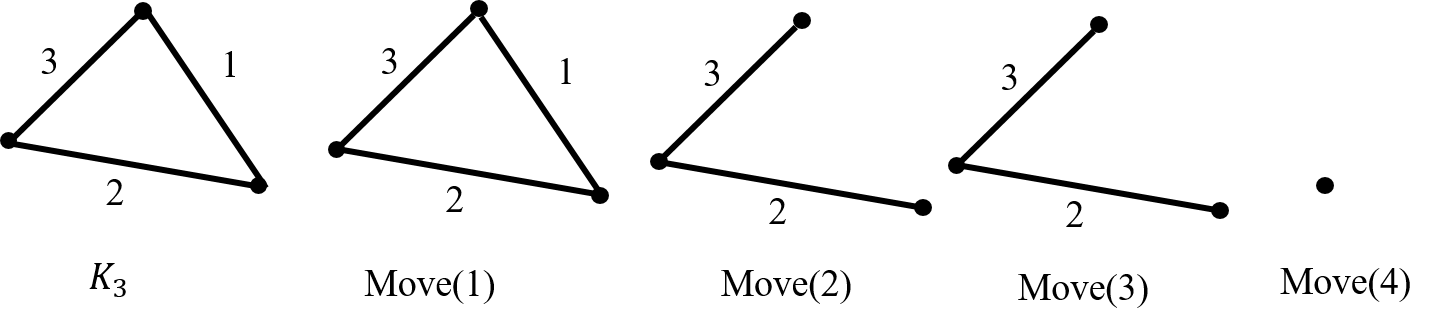
\includegraphics[scale =0.45]{g1.png}
  \caption{The hardness game for graph $K_3$ in Example \ref{exp:hd-K3}.} \label{fig:hd1}
  \end{center}
  \end{figure}
\end{examp}

\begin{examp}\label{exp:hd-K4}
Fig \ref{fig:game2} shows the Prover-Delayer game based on optimal atomic move in Lemma \ref{lem:atmvtseitin} for graph $K_4$ in Fig \ref{fig:hd2}. Delayer starts the game and since the graph has no bridge, Delayer takes no action. Then, Prover removes an edge (in this case, he can remove any edge). In third move, Delayer again takes no action since there is no bridge. Then, Prover whether removes edges 1 or 4 (in this case we continue with removing edge 1) the result would be the same. In next move, Delayer has to remove edge 6 (the bridge) and divides the graph into two components: one isolated vertex and the graph $K_3$. Delayer keeps the bigger component (graph $K_3$) and the rest of the game would be the same as Example \ref{exp:hd-K3}. Thus, we get $\hardness(K_4)=4$.
  \begin{figure}%[h]
  \centering
  \begin{tabular}{|c|c|} 
  \hline
                  Delayer & Prover \\ \hline
                  empty move & removing edge 2  \\ \hline
                  empty move & removing edge 1  \\ \hline
                  removing edge 6 and discarding the vertex & removing edge 5  \\ \hline
                  empty move & removing edge 4 and keeping the vertex\\ \hline
  \end{tabular}
  \caption{The optimal atomic moves for Fig \ref{fig:hd2} and  $\hardness(K_4)=4$.} \label{fig:game2}
  \end{figure}
  \begin{figure}
  \begin{center}
  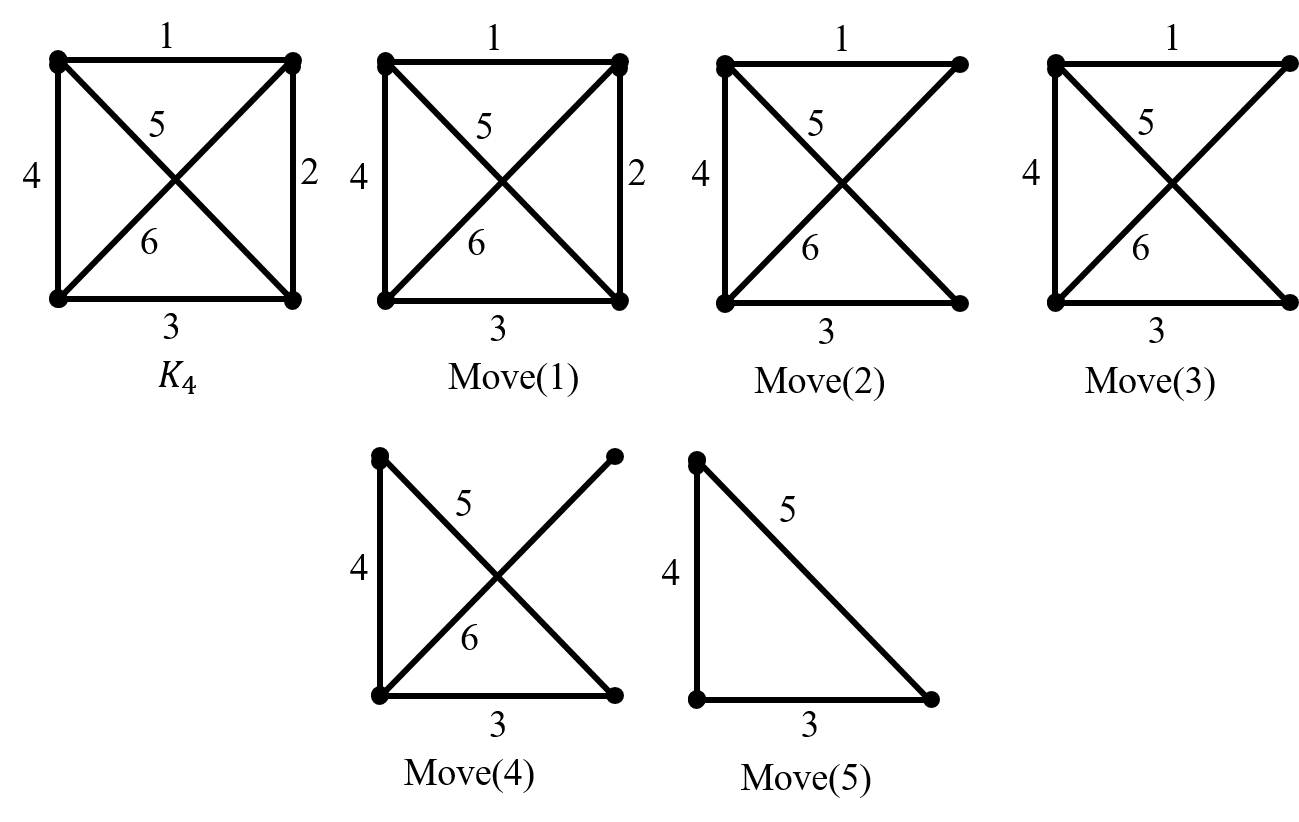
\includegraphics[scale =0.26]{g2.png}
  \caption{The hardness game for graph $K_4$ in Example \ref{exp:hd-K4}.}  \label{fig:hd2}
  \end{center}
  \end{figure}	   
\end{examp}

\begin{examp}\label{exp:hd-K5}
Fig \ref{fig:game3} shows  the Prover-Delayer game based on optimal atomic move in Lemma \ref{lem:atmvtseitin} for graph $K_5$ in Fig \ref{fig:hd3}. Delayer starts the game and since the graph has no bridge, Delayer performs an empty move. Then, Prover removes an edge (in this case, it can remove any edge). In third move, Delayer again performs an empty move. Then, Prover removes edge 5. Then, the Delayer again chooses to do nothing. In the next move, Prover removes edge 10. Therefore, Delayer has to remove edge 7 (the bridge) and the graph is divided into two components: one separate vertex and the graph $K_4$. Delayer keeps the bigger component (graph $K_4$) and the rest of the game would be the same as Example \ref{exp:hd-K4}. Thus, we get $\hardness(K_5)=7$.
  \begin{figure}%[h]
  \centering
  \begin{tabular}{|c|c|} 
  \hline
                  Delayer & Prover \\ \hline
                  empty move & removing edge 1  \\ \hline
		  empty move & removing edge 5  \\ \hline
		  empty move & removing edge 10  \\ \hline
                  removing edge 7 and discarding the vertex & removing edge 4  \\ \hline
		  empty move & removing edge 3  \\ \hline
                  removing edge 8 and discarding the vertex & removing edge 9  \\ \hline
		  empty move & removing edge 2  and keep the vertex\\ \hline
  \end{tabular}
  \caption{The optimal atomic moves for Fig \ref{fig:hd3} and $\hardness(K_5)=7$.} \label{fig:game3}
  \end{figure}
  \begin{figure}
  \begin{center}
  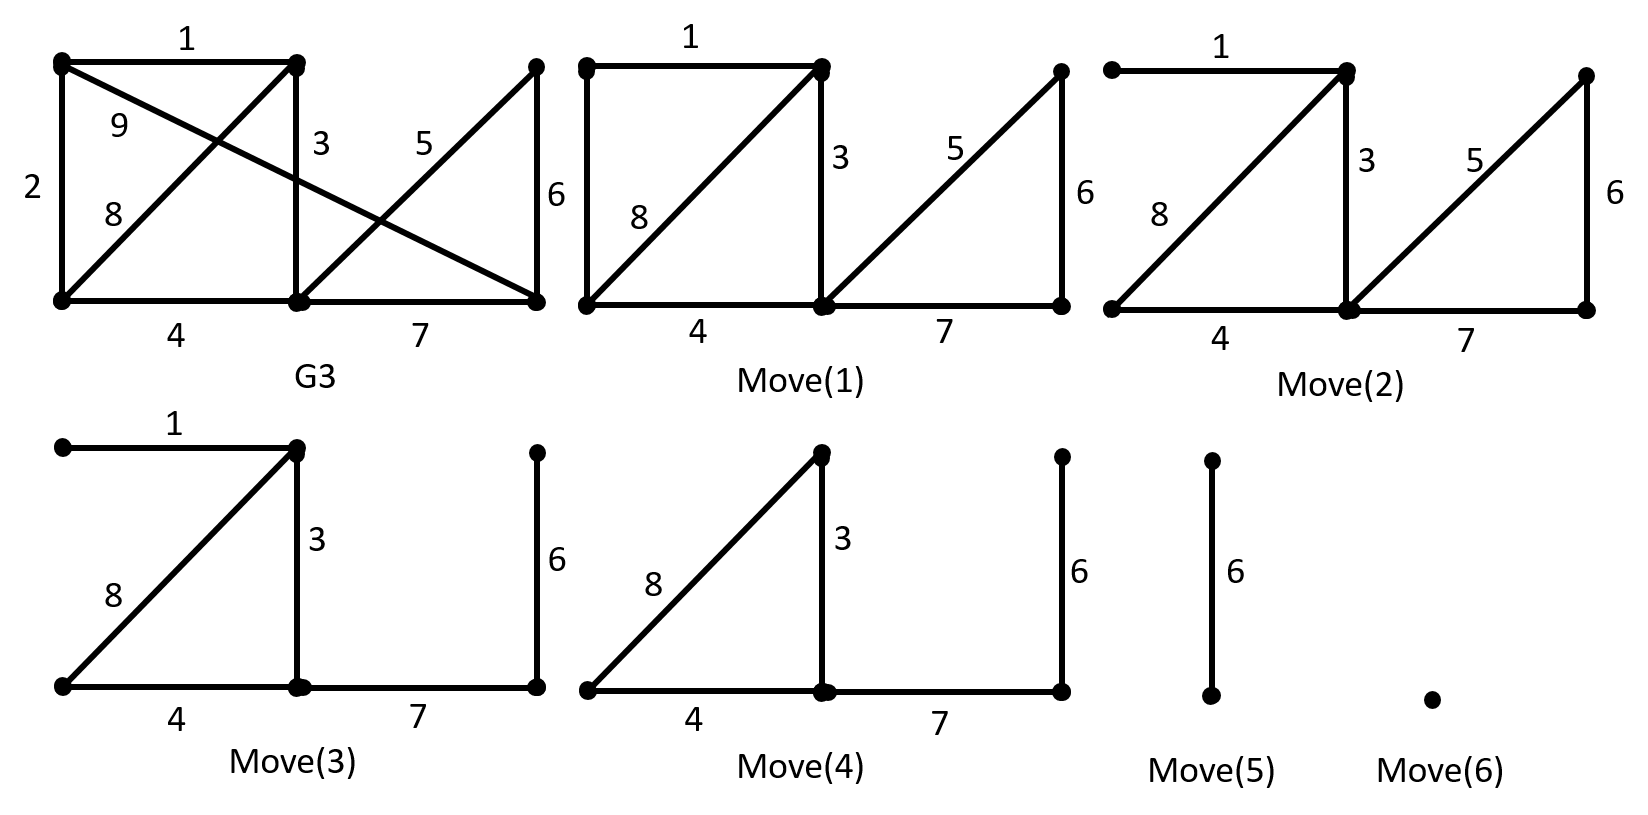
\includegraphics[scale =0.4]{g3.png}
  \caption{The hardness game for graph $K_5$ in Example \ref{exp:hd-K5}.} \label{fig:hd3}
  \end{center}
  \end{figure}
\end{examp}

Based on previous examples, we have Conjecture \ref{con:nobridge-pd} and Lemma \ref{lem:complete-graph}.
\begin{conj}\label{con:nobridge-pd}
If a Tseitin graph $G$ has no bridge and the number of connected edges to vertices are not equal then Prover chooses the vertex with minimum connected edges and removes one of its connected edges.
\end{conj}

%If Conjecture \ref{con:nobridge-pd} is true, then we have the following lemma:	  
\begin{lem}\label{lem:complete-graph}
Consider a non-trivial complete graph $K_n, n \in \NN$ as a Tseitin graph. Then, we have $\hardness(K_n)= n-2+\hardness(K_{n-1})$. 
\end{lem}	
\begin{prf}
In a complete graph $K_n$, there are $n-1$ connected edges to each vertex. At first, if $n =2$ then the graph has one edge. In this case, Delayer does not remove the edge (since the game ends) and Prover gets one point by removing that edge. Else, there is no bridge and Delayer does not remove any edge. Then, Prover chooses a vertex and removes a connected edge of that vertex. Now, there are only two cases. The first case is that there is only one edge (we get graph $K_2$) and again Delayer differ the choice to Prover. The second case is that there is no bridge and Prover continues the game by removing one connected edge of the vertex with minimum number of connected edges (based on Conjecture \ref{con:nobridge-pd}). This process continues till there is only one bridge that connects a vertex to the graph $K_{n-1}$. In this case, Delayer removes the bridge and chooses the graph $K_{n-1}$. Thus, we have $\hardness(K_n)= (n-1)-1+\hardness(K_{n-1}) $. Table \ref{fig:table1} shows $\hardness(K_n)$ for some $n$.
   \begin{figure}[h]
   \centering
   \begin{tabular}{|c|c|} 
                  \hline
                  $n$ & $\hardness(K_n)$ \\ \hline
		  2 & 1  \\ \hline
		  3 & $1+ \hardness(K_2)=2$ \\ \hline
		  4 & $2+ \hardness(K_3)=4$  \\ \hline
	   	  5 & $3+ \hardness(K_4)=7$  \\ \hline
		  6 & $4+ \hardness(K_5)=11$  \\ \hline
		  7 & $5+ \hardness(K_6)=16$  \\ \hline
   \end{tabular}
   \caption{The hardness for complete graph $K_n$.}  \label{fig:table1}
   \end{figure}
\end{prf}

\begin{lem}\label{lem:graphwithcomplt}
Consider the game in Lemma \ref{lem:game-tseitin-hd} for a Tseitin graph $G$. During the game, if we obtain a complete graph $K_n, n \in \NN$, then the hardness would be the sum of Prover's points (until that step) and $\hardness(K_n)$.
\end{lem}	
\begin{prf}
Based on Lemma \ref{lem:game-tseitin-hd} and \ref{lem:complete-graph}.
\end{prf}
  
\begin{examp}\label{exp:graph-notK}
Fig \ref{fig:game4} shows the atomic moves of hardness game for graph $G_1$ in Fig \ref{fig:hd4}. In first move, the graph has no bridge and Delayer performs an empty move. Then, Prover chooses a vertex with the least number of connected edges and removes one of its edges (edge 5). In next move, the graph has a bridge (edge 6) and removes the bridge and discards the smaller component (the isolated vertex). Then, Prover chooses another vertex with the least number of connected edges and removes one of its edges (edge 9). Delayer, again, finds a bridge (edge 7) and removes it. Then, Prover removes edge 3 and in next move, Delayer removes the bridge (edge 4). In this step, the left component is graph $K_3$ and the rest of game is the same as Example \ref{exp:hd-K3}. Thus, we get $\hardness(G_1)=3+\hardness(K_3)=5$.
  \begin{figure}[h]
  \centering
  \begin{tabular}{|c|c|} 
  \hline
                  Delayer & Prover \\ \hline
                  empty move & removing edge 5  \\ \hline
		  removing edge 6 and discarding the vertex & removing edge 9  \\ \hline
		  removing edge 7 and discarding the vertex & removing edge 3  \\ \hline
		  removing edge 4 and discarding the vertex & removing edge 8  \\ \hline
		  empty move & removing edge 2  and keeping the vertex\\ \hline

   \end{tabular}
   \caption{The optimal atomic moves for Fig \ref{fig:hd4}.} \label{fig:game4}
   \end{figure}
   \begin{figure}
   \begin{center}
   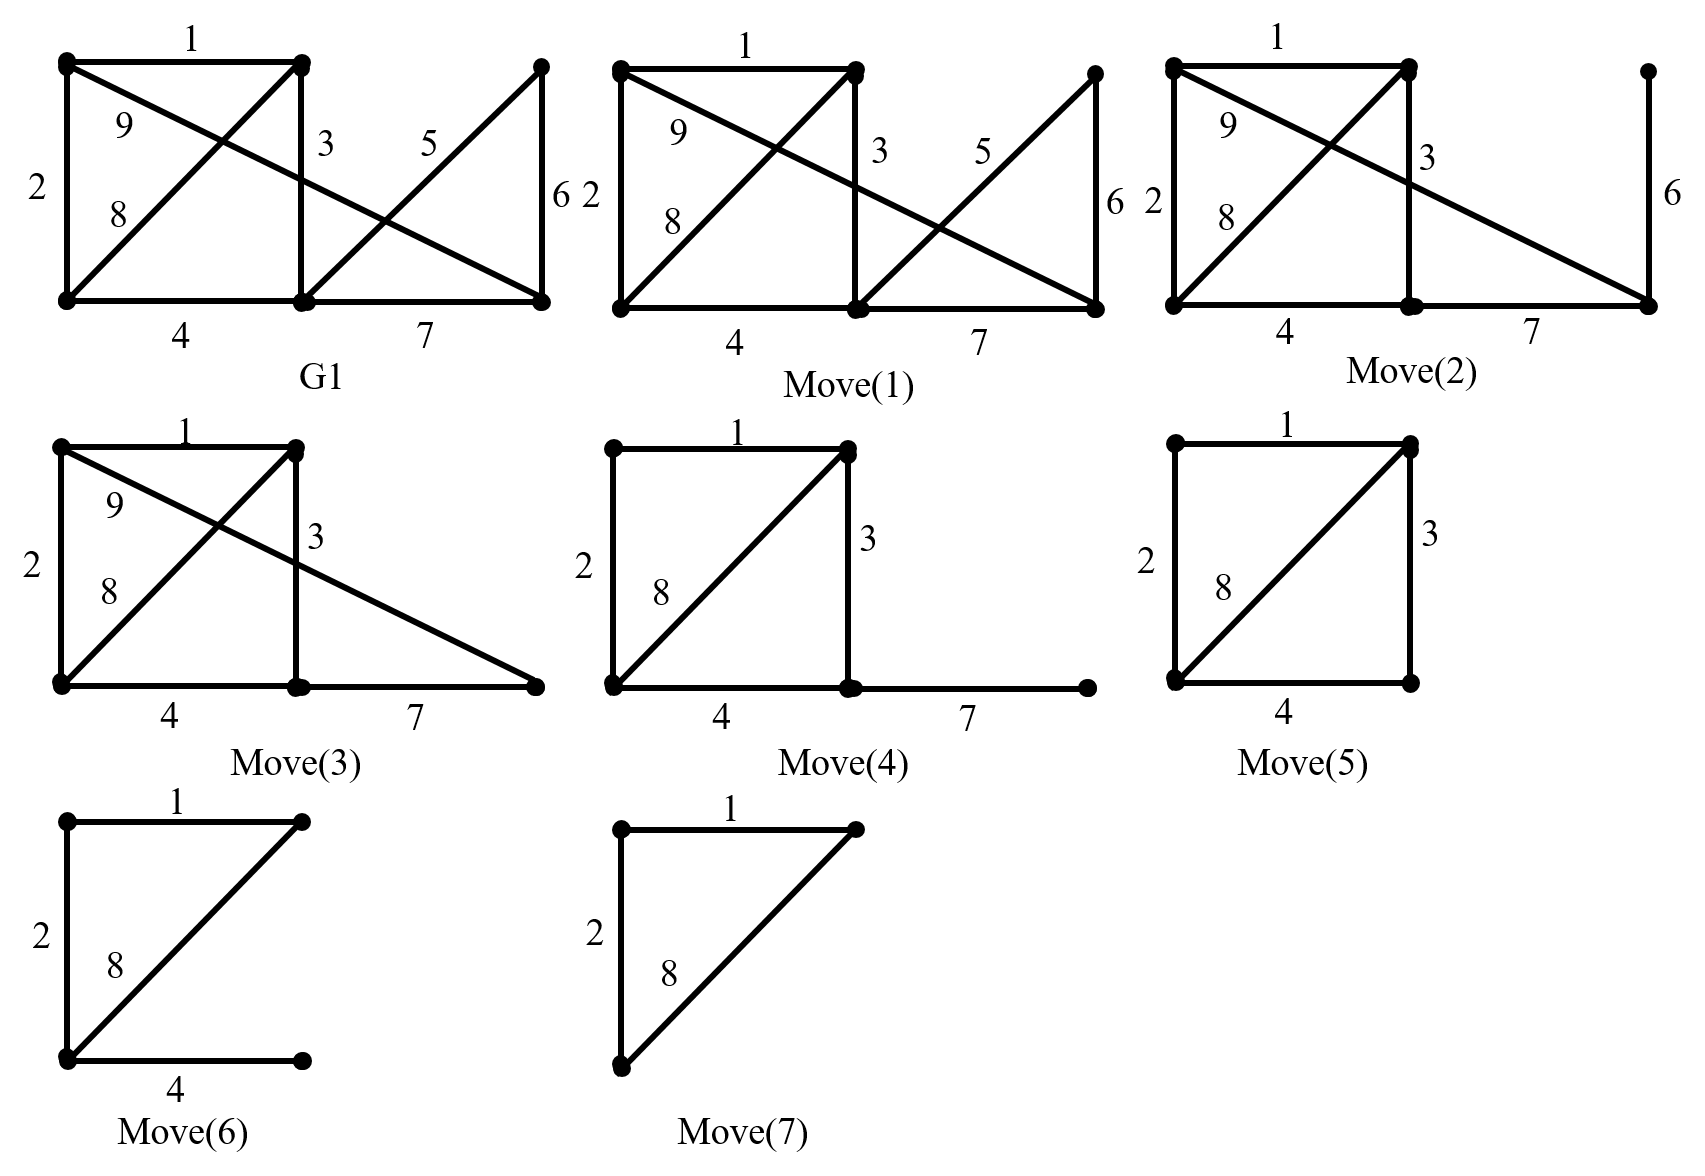
\includegraphics[scale =0.4]{graph_hd1.png}
   \caption{The hardness game for graph $G_1$ in Example \ref{exp:graph-notK}.}  \label{fig:hd4}
   \end{center}
   \end{figure}
\end{examp}
  
\begin{conj}\label{con:hd_game2}
For all Tseitin graphs $G$ with $n$ vertices, graph $K_n$ has the worst case of the hardness (the maximum of $\hardness$) which is equal to $\hardness(K_n)= n-2+\hardness(K_{n-1})$ according to Lemma \ref{lem:complete-graph}.
\end{conj}

\begin{conj}\label{con:hd-game-time}
The time complexity of the Delayer-Prover game in Lemma \ref{lem:game-tseitin-hd} is polynomial time.
\end{conj}

\begin{quest}\label{que:gamehd-move}
Consider Lemma \ref{lem:game-tseitin-hd} for a Tseitin graph $G$. If Delayer removes some non-bridge edges $e \in E$ such that the hardness remain unchanged, then is optimal value of the game still the hardness of $G$?
\end{quest}

\begin{quest}\label{que:gamehd}
How can we extend the game in Lemma \ref{lem:game-tseitin-hd} for Tseitin hypergraph (which is defined as full Tseitin graph in \cite{BeyersdorffGwynneKullmann2013PHPER})?
\end{quest}

%%%%%%%***********************************
In Section  \ref{sec:game-whdf}, a game characterisation is given to obtain the width-hardness of a clause-set $F \in \Usat$. Here, this game is applied to a Tseitin garph $G$ based on Lemma 9.7 in \cite{BeyersdorffGwynneKullmann2013PHPER}.

\begin{lem}\label{lem:whd-tseitin-game}
By \cite{BeyersdorffGwynneKullmann2013PHPER}, consider  a Tseitin graph $G$ for a Tseitin clause-set $T(G,\rho) \in \Usat$. Then $\whardness(T(G,\rho))$ is obtained as follows:
  \begin{enumerate}
  \item The atomic move is the same as Lemma \ref{lem:game-tseitin-hd} (as removing some $e \in E(G)$ and choosing a connected component of $G - e$).
  \item Two players play in turns, and Delayer starts the game.
  \item A move of Delayer is to apply a sequence of atomic moves (possibly zero).
  \item A move of Prover is to replace the current global sequence of atomic moves by another sequence, which is consistent with the old sequence, and handles exactly one new edge (that is Prover can undo some of Delayer's atomic moves in the history of the game).
  \item Here ``consistent'' means that in case of removing a bridge, the same component of the graph is chosen.
  \item The games ends when $G$ becomes trivial, in this case Delayer gets as many points as the maximum length of a sequence used in a replacement by Prover (which is equal $\whardness(T(G,\rho))$).
  \end{enumerate}
\end{lem}

\begin{conj}\label{con:whd-gametime}
The time complexity of the Delayer-Prover game in Lemma \ref{lem:whd-tseitin-game} is polynomial time.
\end{conj}

\begin{quest}\label{que:game-whd-atm}
What are the optimal atomic moves for the players in Lemma \ref{lem:whd-tseitin-game}?
\end{quest}

\begin{quest}\label{que:game-whd-Kn}
Consider Lemma \ref{lem:whd-tseitin-game}. Can we obtain a formula for $\whardness(T(G,\rho))$ of complete Tseitin graph $G$?
\end{quest}

%%%%%%%%%%%%%%%%%%%%%%%%%%%%%%%%%%%%%%%%%%%%%%%%%%%%%%%%%%
\chapter{Structure of minimally unsatisfiable clause-sets}
\label{cha:mucls}

\section{Background}
\label{sec:basicdef}

In this section, an overview of minimally unsatisfiable clause-sets is given at first. Then, special reduction/extension with application for minimally unsatisfiable clause-sets is explained. Finally, the deficiency of clause-sets is used as a measure for classification of minimally unsatisfiable clause-sets which is already investigated in \cite{KullmannZhao2010Extremal, Kullmann2007HandbuchMU, KullmannZhao2016UHitSAT, KleineBuening2000SubclassesMU, Ku99dK} but in this report, more details are discussed.
%One of the main class of unsatisfiable clause-sets are minimally unsatisfiable clause-sets which is referred as the building block for understanding unsatisfiability in \cite{KullmannZhao2010Extremal}. So, understanding the concept of minimally unsatisfiable clause-sets and investigating their properties and subclasses are important. An overview of these clause-sets are presented in \cite{KullmannZhao2010Extremal, Kullmann2007HandbuchMU,KullmannZhao2012ConfluenceJ}. An interesting measure for the complexity of clause-sets and particularly minimally unsatisfiable clause-sets is deficiency. 

\begin{defi}\label{def:mu}
A clause-set $F \in \Usat$ is \textbf{minimally unsatisfiable} if by removing any arbitrary clause $C \in F$, the clause-set $F \sm \set{C}$ becomes satisfiable. The set of all minimally unsatisfiable clause-sets is indicated by $\bmm{\Musat} \in \Usat$.
\end{defi}
Remarks:
  \begin{enumerate}
  \item The complexity of the problem $\Musat \in \Usat$ is $D^P$-complete (by Theorem 11.1.1 in \cite{Kullmann2007HandbuchMU}).
  \item All full clause-sets $ A_n$ are in $\Musati{}$.
  \end{enumerate}

\begin{defi}\label{def:deficiency}
The \textbf{deficiency} for a clause-set $F \in \Cls$ is defined as the difference between the number of clauses and the number of variables and indicated by $\bmm{\delta} \in \ZZ: \delta(F)= c(F) - n(F)$.
\end{defi}
Remarks:
  \begin{enumerate}
  \item In this report, the minimally unsatisfiable clause-sets with deficiency $k \in \ZZ$ are indicated by $\Musati{\delta=k}$.
  \item The complexity of the problem $\Musati{\delta=k}$ with fixed $k$ is $P$ (by Theorem 11.2.1 in \cite{Kullmann2007HandbuchMU}).
  \item All $F \in \Musati{\delta=k}$ have $k \ge 1$ (by Theorem 8 in \cite{DDK98}).
  \end{enumerate}

\begin{defi}\label{def:degree}
For a clause-set $F \in \Cls$ the \textbf{literal degree} for a literal $x \in \lit(F)$ is the number of the literal occurrence and denoted by $\bmm{\ldeg_F(x)} \in \NNZ$. The \textbf{variable degree} for a variable $v \in \var(F)$ is defined as $\bmm{\vdeg_F(v)} := \ldeg_F(v) + \ldeg_F(-v) \in \NNZ$. Also, the \textbf{minimum variable degree} (or min-var-deg) is defined as the minimum of variable degree for all variables in $F$ and indicated by $\bmm{\minvdeg(F)} \in \NN$.
\end{defi}
Remarks:
  \begin{enumerate}
  \item It is obvious that $\vdeg_F(v) \le 2 \delta(F)$ and thus for $n(F) >0$, $\minvdeg(F) \le 2 \delta(F)$. A sharper upper bound for $\minvdeg(F)$ is given in Theorem 9.10 of \cite{KullmannZhao2010Extremal}.
  \item All full clauses $A_n$ have deficiency $2^n - n$ and if $n \ge 1$, then  $\minvdeg(A_n) =2^n$.
  \item In \cite{KullmannZhao2010Extremal}, the problem of finding the min-var-deg for minimally unsatisfiable clause-sets with fixed deficiency is indicated by $\minnonmer(k) $ (that is $\minnonmer(k)  :=  \minvdeg(\Musati{\delta=k}) \in \NN$) and an improved upper bound/ lower bound for $\minnonmer(k) $ is given.
    \end{enumerate}
    
\begin{defi}\label{def:singvar}
By \cite{KullmannZhao2012ConfluenceJ}, for a non-pure variable $v \in \var(F)$ if $\min(\ldeg_F(v) ,\ldeg_F(-v))=1$, then it is called a \textbf{singular variable}. If a clause-set $F$ does not have any singular variable, it is called \textbf{nonsingular}. An \textbf{m-singular variable} is a singular variable with $\vdeg_F(v)=m+1$, $m \in \NN$.
\end{defi}
Remarks:
  \begin{enumerate}
  \item The set of nonsingular minimally unsatisfiable clause-sets $F \in \Musat$ is indicated by $\bmm{\Musat'} \in \Musat$. Thus, if $F \in \Musat'$, then all variables in $F$ are occurred at least twice positively and at least twice negatively.
  \item A \textbf{non-1-singular variable} is a variable which $m$-singular for some $m \ge 2$.
   \end{enumerate}
 
\begin{defi}\label{def:splitting}
For $F \in \Cls$, consider a variable $v \in \var(F)$. \textbf{Splitting} of $F$ on $v$ is the process of obtaining two clause-set $F_0,F_1$ such that  $F_0:=\pao v0 * F$ and $F_1:=\pao v1 * F$.
\end{defi}
Remarks:
  \begin{enumerate}
  \item For $F \in\Musati{\delta=k}$, splitting may lead to produce two minimally unsatisfiable clause-sets $F_0,F_1$ but generally one can not speak of minimally unsatisfiability unless more information is provided. 
  \item For $F \in\Musatnsi{\delta=k}$ if after splitting on a variable $v \in \var(F)$ the clause-sets $F_0,F_1$ are minimally unsatisfiable with deficiency $k_0, k_1$, then we have $k_0, k_1 < k$ (by Theorem 2 in \cite{KleineBuening2000SubclassesMU}).
  \item For $F \in \Musat$, the application of splitting for $\delta=2$ are investigated in Sections \ref{sec:smu2}.
  \end{enumerate}
%-----------------------------------------------------------------------------
\section{Autarkies}
\label{sec:autrk}

\begin{defi}\label{def:autarky}
For a clause-set $F \in \Cls$ a partial assignment $\vp \in \Pass$ is called an  \textbf{autarky} if $\fa\, C \in F : \vp * \set{C} \in \set{\set{C}, \top}$. That is whenever a clause is touched by an autarky $\vp$, then it is satisfied.
\end{defi}
Remarks:
  \begin{enumerate}
  \item If $\vp \in \Pass$ is an autarky for $F \in \Cls$, then the application of $\vp *F$ is sat-equivalent for $F$. 
  \item All satisfying assignment for $F$ are autarky.
  \item The empty partial assignment $\epa$ is an autarky for every $F \in \Cls$ and more generally all $\varphi \in \Pass$ with $\var(\varphi) \cap \var(F) = \emptyset$ are autarkies for $F$. 
  \item An autarky $\vp$ for $F$ is called \textbf{trivial} if $\var(f) \cap \var(\vp) = \es$. Else, it is called a \textbf{non-trivial} autarky.
  \item A clause-set with no non-trivial autarky is called a \textbf{lean clause-set}. The set of all lean clause-sets is denoted by $\bmm{\Lean} \subset \Usat \addcup \set{\top}$. An overview on autarkies and lean clause-sets are given in \cite{Ku00f, Kullmann2007HandbuchMU}. 
  \end{enumerate}
  
\begin{defi}\label{def:autarky-redc}
If $\vp \in \Pass$ is a non-trivial autarky for a clause-set $F \in \Cls$, then $\vp *F$ is called \textbf{autarky reduction} for $F$ (and is sat-equivalent to $F$).
\end{defi} 
Remarks:
  \begin{enumerate}
  \item If we apply all possible autarky reduction for a clause-set $F$, then we get the \textbf{lean kenrel} of $F$ (Section 11.8.3 in \cite{Kullmann2007HandbuchMU} provides more details of lean kernel). The lean kernel is the largest lean sub-clause-set of $F$.
  \item Another equivalent description for lean clause-sets according to \cite{Ku00f} is that if $F \in \Lean \sm \top$ then every clause $C \in F$ is used in at least one resolution refutation for $F$. Thus, the lean kernel of $F$ is the set of all clauses from $F$ that can be used in at least one resolution refutation for $F$ (by Theorem 11.8.1 in \cite{Kullmann2007HandbuchMU}).
  \item The autarky reduction is obtained in a polynomial time, but finding the autarky in polynomial time is still an open question (\cite{KullmannZhao2010Extremal} in Section 10.1 discusses whether the autarky can be found in polynomial time).
  \end{enumerate}
%-----------------------------------------------------------------------------
\section{Hitting clause-sets}
\label{sec:hit}

\begin{defi}\label{def:hit-cls}
A clause-set $F \in \Cls $ is called a \textbf{hitting clause-set} iff all clauses $C,D \in F$, $C \not = D$ have at least one clash. The set of all hitting clause-sets is indicated by $\bmm{\Clash} \in \Cls$.
\end{defi}
Remarks:
  \begin{enumerate}
  \item The set of all unsatisfiable hitting clause-sets is indicated by $\bmm{\Uclash} := \Usat \cap \Clash$. The set of all nonsingular unsatisfiable hitting clause-sets is denoted by $\bmm{\Uclash'} \subset \Uclash$).
  \item If $F \in \Uclash$, then every clause $C \in F$ (as a partial assignment) is a satisfying assignment for $F \sm \set{C}$.
  \item If $F \in \Musat$ then removing any clause $C \in F$ makes $F \sm \set{C}$ satisfiable. On the other hand, if $F \in \Uclash$ then every $C \in F$ is a satisfying assignment for $F \sm \set{C}$. Thus, $\Uclash \subset \Musat$. \cite{KullmannZhao2016UHitSAT} gives an overview of unsatisfiable hitting clause-sets.
  \item For all full clauses $A_n$ we have $A_n \in \Uclash$.
  \end{enumerate}

 \begin{defi}\label{def:nhit-cls}
A clause-set $F \in \Cls $ is called a \textbf{nearly-hitting clause-set} iff for all clauses $C,D \in F$, $C \not = D$ either $\var(C) \cap \var(D) = \es$ or $C,D$ have at least one clash. The set of all nearly-hitting clause-sets is denoted by $\bmm{\Nclash} \subset \Cls$.
\end{defi}
Remarks:
  \begin{enumerate}
  \item If $F \in \Nclash$, then every $C \in F$, as partial assignment, is an autarky for $F \sm \set{C}$.
  \end{enumerate}
  
\begin{quest}\label{ques:nhit-sat}
The complexity of SAT-decision for nearly-hitting clause-sets is open (also in the boolean case).
\end{quest}   
 %-----------------------------------------------------------------------------              
\section{Saturated minimally unsatisfiable clause-sets}
\label{sec:smu}

\begin{defi}\label{def:smu}
A clause set $F \in \Cls$ is called \textbf{saturated} minimally unsatisfiable iff $F \in \Musat $ and by replacing any $C \in F$ by any super-clause $C' \supset C$, the result clause-set is satisfiable. The set of all saturated minimally unsatisfiable clause-sets is denoted $\bmm{\Smusat} \subset \Musat$.
\end{defi}
Remarks:
  \begin{enumerate}
  \item The set of all nonsingular saturated minimally unsatisfiable clause-sets is indicated by $\bmm{\Smusatns} \subset \Smusat$.
  \item For all clause-sets $F \in \Cls$, if $F \in \Uclash$ then $ F \in \Smusat$ ,i.e. $\Uclash \subset \Smusat$ (by Lemma 2 in \cite{KullmannZhao2012ConfluenceJ}). 
  \item The properties of clause-set in $\Smusatnsi{\delta=1}, \Smusatnsi{\delta=2}$ are investigated in Sections \ref{sec:smu1} , \ref{sec:smu2}.
  \item For every $F \in \Musat$ there is a saturation $F' \in \Smusat$. A saturated clause-set  $F'$ for $F$ is obtained using an operation defined in Definition \ref{def:smu-opr}.
  \end{enumerate}

\begin{defi}\label{def:smu-opr}
\cite{KullmannZhao2012ConfluenceJ} For every $F \in \Musat$ a saturation $F' \in \Smusat$ is obtained by iterated application of the operation $\saturate(F,C,x)$ as follows where $C \in F$, $x \in \lit(F)$ and $\var(x) \not \in \var(C)$:
  \begin{displaymath}
    \bmm{\saturate(F,C,x)} := (F \sm \set{C}) \cup (C \addcup \set{x}) \in \Cls
  \end{displaymath}
If in iteration $m$ there is no literal in $F$ fulfilling the conditions $\var(x) \not \in \var(C)$ for all clauses of $F$ and $F_m \in \Usat$, then $F' =F_m=\saturate(F_{m-1},C_{m-1},x_{m-1}) \in \Smusat$. 
\end{defi}
Remarks:
  \begin{enumerate}
  \item If $F' \in \Smusat$ is a saturation for $F \in \Musat$, then we have $n(F')=n(F)$, $c(F')=c(F)$ and $\delta(F')=\delta(F)$.
  \item If $C \in F$ and $\var(C) = \var(F)$ (full clause), then no literal can be added to $C$ to make $F$ saturated. Also, all full clauses $A_n$ are in $\Smusat$.
  \item By \cite{Ku99dK}, we have $ \Smusati{\delta=k} \subset \Musati{\delta=k} \subset \Lean_{\delta=k} \subset \Usat_{\delta=k} \cup \set{\top} $ which are poly-time decidable.
  \end{enumerate} 
  
\begin{examp}\label{exp:smu-exp}
 For $F = \set{\set{a,b},\set{\ol{a}},\set{\ol{b}}} \in \Musat \sm \Smusat$ using the Definition \ref{def:smu-opr} we can have $F'=\set{\set{a,b},\set{\ol{a},b},\set{\ol{b}}} \in \Smusat$ or $F'=\set{\set{a,b},\set{\ol{a}},\set{a,\ol{b}}} \in \Smusat$.
\end{examp}

\begin{lem}\label{lem:smu-mu}
By \cite{KullmannZhao2010Extremal}  $F' \in \Smusat$ iff for all $v \in \var(F)$, $\langle v \ra 1 \rangle*F \in \Musat$.
\end{lem}

\begin{lem}\label{lem:smu-app}
By \cite{KullmannZhao2010Extremal}, consider a clause-set $F \in \Smusat$. If $F$ is a full clause-set and also it is the saturation of some $F' \in \Musat$, then $F' = F$. Otherwise, if $F$ is not a full clause-set then there exist some some $F' \in \Musat$ with $F' \not= F$ such that $F$ is a saturation of $F'$.
\end{lem}

\begin{quest}\label{que:smu-elim}
For a clause-set $F \in \Smusat$ if $F'$ is obtained by eliminating a literal occurrences in $F$, is $F'$ still minimally unsatisfiable? (that is for $C \in F$, $x \in C$, whether $F' := (F \sm \set{C}) \addcup \set{C \sm \set{x}}$ is in $\Musat$ ?)
\end{quest}
%-----------------------------------------------------------------------------
\section{Reduction/ extension of minimally unsatisfiable clause-sets}
\label{sec:r-e}

To understand the structure of minimally unsatisfiable clause-sets and finding the isomorphic types of $\Musati{\delta=k}$ some types of reduction/ extension of clause-sets are reviewed in this section according to \cite{KullmannZhao2010Extremal,KullmannZhao2012ConfluenceJ}.

\subsection{Singular reduction/ extension}
\label{sec:sing-re} 

\begin{defi}\label{def:singularDP}
Consider DP-reduction in Definition \ref{def:dpredc}. If a DP-reduction is performed for a singular variable, then it is called a \textbf{singular DP-reduction} and the set of all nonsingular clause-sets obtainable from $F$ by singular DP-reduction denoted by $\bmm{sDP(F)}$. 
\end{defi}
Remarks:
  \begin{enumerate}
  \item Base on Lemma 5.3 in \cite{KullmannZhao2010Extremal}, if a clause-set $F$ is minimally unsatisfiable then after performing the singular DP-reduction, the result clause-set $F'$ is also minimally unsatisfiable. This is also true when $F$ is in $\Smusat$ or $\Uclash$.   Further more, the singular DP-reduction does not change the deficiency of $F$ since $c(F)$ and $n(F)$ both decreased by one (an overview of DP-reduction for minimally unsatisfiable clause-sets is presented in \cite{KullmannZhao2012ConfluenceJ}).
  \item If $F \not \in \Musat$, then after singular DP-reduction the result is also not minimally unsatisfiable.
  \item For $F \in \Musat$, the application of $sDP$ for $\delta=1$ and $\delta=2$ are investigated in Sections \ref{sec:smu1} and \ref{sec:smu2}.
  \end{enumerate}
  
\begin{lem}\label{lem:sDP-infl}
For a clause-set $F \in \Musati{\delta=k}$:
  \begin{enumerate}
  \item If $k=1$, then an iterated application of singular DP-reduction leads to $\set{\bot}$ (that is $sDP(F)=\set{\bot}$).
  \item If $k \ge 2$, then an iterated application of singular DP-reduction leads to a clause-set in $\Musatnsi{\delta=k}$ (by Lemma 1 in \cite{KleineBuening2000SubclassesMU}).
  \end{enumerate}
\end{lem} 

\begin{lem}\label{lem:sDP-size}
By \cite{KullmannZhao2012ConfluenceJ}, for $S \in \Smusat$ we have $\abs{\sdp(F)} = 1$.
\end{lem} 

\begin{defi}\label{def:singularextn}
By \cite{KullmannZhao2010Extremal} for a clause-set $F \in\Cls$ and a variable $v \not \in \var(F)$, a \textbf{singular extension} is defined as the reverse direction of a singular DP-reduction. Thus, for obtaining a \textbf{singular m-extension} $F' $of $F$ with $v$, first we choose $m$ different clauses $D_i:D_1, \dots, D_m \in F$. Then, we consider a clause  $C: C \sse \bca_{i=1}^m D_i$. In the next step, for every $D_i$ we consider a clause $D_i':(D_i \sm C) \sse D_i' \sse D_i$. Finally, we obtain $C' := C \addcup \set{x}$, and $D_i'' := D_i' \addcup \set{\ol{x}}$ for $i \in \tb 1m$. Then, we have:
  \begin{displaymath}
    F' := (F \sm \set{D_1,\dots,D_m}) \addcup \set{C', D_1'',\dots,D_m''}.
  \end{displaymath}
\end{defi}
Remarks:
  \begin{enumerate}
  \item Consider an $m$-extension $F'$ of $F$. Then, $F \in \Musat \iff F' \in \Musat$ (by Lemma 5.9 in \cite{KullmannZhao2010Extremal}).
  \item The singular m-extension of $F$ does not change the deficiency of $F$. But, number of clauses (and variables) is increased by one.
  \end{enumerate}
  
\begin{defi}\label{def:unit-ext}
By \cite{KullmannZhao2010Extremal} for a clause-set $F \in \Cls$, a \textbf{full singular unit-extension} $F' \in \Cls$ is obtained as follows: First, consider a literal $x:\var(x) \notin \var(F)$. Then, $F' := \set{\set{x}} \addcup \set{C \addcup \set{\ol{x}} : C \in F}$. Thus, $F' $ has a unit clause $\set{x}$ and all clauses of $F$ with literal $\ol{x}$ added to them.
\end{defi}
Remarks:
  \begin{enumerate}
  \item Consider $F'$ as the full singular unit-extension of $F$, if $F \in \Musati{\delta=k} $ the  $F' \in \Musati{\delta=k} $. This is also true about $F \in \Smusati{\delta=k}$. (by Lemma 5.17 in \cite{KullmannZhao2010Extremal}).
  \end{enumerate}
%-----------------------------------------------------------------------------
\subsection{Full subsumption resolution/ extension}
\label{sec:fsr-e}  

\begin{defi}\label{def:sres}
The \textbf{subsumption resolution} is a reduction of a clause-set $F \in \Cls$ to $F' \in \Cls$ by removing a literal $x : \var{x} \in \var{F}$ from a clause $C:C \in F$ when there is a clause $D \in F: \ol x \in D$ and also $D \sm \set{\ol x} \sse C$. This means that the resolution of $C,D$ subsumes $C$. Note that $D$ is still in $F'$.
\end{defi}

\begin{defi}\label{def:fsr}
\cite{KullmannZhao2010Extremal} The \textbf{strict full subsumption resolution} is the reduction of $F \in \Cls$ to $F'\in \Cls$ as follows and indicated by $\bmm{F \tsubres F'}$. To obtain $F'$, consider a clause $R \in F'$ (the resolvent) and a literal $x \in \var(F'):\var(x) \notin R$ ($x, \ol{x}$ the resolution literals). Then if $C := R \addcup \set{x}$ and $D := R \addcup \set{\ol{x}}$ (the parent clauses), then we have $F = (F' \sm \set{R}) \addcup \set{C,D}$.

$F \tsubresk{k} F'$ for $k \in \NNZ$ shows the application of exactly $k$ steps of strict full subsumption resolution. 
\end{defi}
   
\begin{defi}\label{def:fse}
Based on \cite{KullmannZhao2010Extremal} the \textbf{strict full subsumption extension} in the reverse direction of the strict full subsumption resolution. Thus by considering the parameters in Definition \ref{def:fsr} for $F, F'$ and $F \tsubres F'$, the clause $R$ is expanded to $C = R \addcup \set{x}$, $D = R \addcup \set{\ol{x}}$ and we say $F$ is obtained from $F'$ by strict full subsumption extension.
\end{defi}
Remarks:
  \begin{enumerate}
  \item If  $F \tsubres F'$ and $F \in \Musat $ then $ F' \in \Musat$ and also if $F \in \Smusat$ we have $ F' \in \Smusat$ while if $ F' \in \Smusat$ then $F \in \Musat $ ( by Lemma 6.5 in \cite{KullmannZhao2010Extremal}). 
  \item Note that for the full subsumption resolution/ extension for the resolution variable $v$, if $v$ is occurred in other clauses then it is called \textbf{strict} but if the variable is vanished it is called \textbf{non-strict}.
  \end{enumerate}
%-----------------------------------------------------------------------------
\section{Classification of minimally unsatisfiable clause-sets}
\label{sec:c-mucls}

Considering definitions and tools given in previous sections, minimally unsatisfiable clause-sets can be classified based on their deficiencies. In Section \ref{sec:smu1}, a comprehensive overview on the clause-sets in $\Musati{\delta=1}$ with some new results are presented. Then, a formula for every $F' \in \Musatnsi{\delta=2}$ is given in Section \ref{sec:smu2} and some new properties of $F \in \Musati{\delta=2}$ are obtained. Finally, the clause-sets in $ \Musati{\delta=3}$ are investigated in Section \ref{sec:smu3} and some questions regarding minimally unsatisfiable clause-sets with $\delta \ge 3$ are discussed. 

\begin{lem}\label{lem:mu-refu-tree}
Based on \cite{KleineBuening2000SubclassesMU} if $F \in \Musati{\delta=k}$ then an iterated application of singular DP-reduction and the splitting leads to a splitting tree, where the leafs are labeled with clause-sets in $\Musati{\delta=1}$. Also, the number of leafs of the splitting tree is bounded by $2^{k-1}$.
\end{lem}
%-----------------------------------------------------------------------------  
\subsection{Structure of $\Musati{\delta=1}$}
\label{sec:smu1}

\begin{lem}\label{lem:mu1-uvd}
\cite{KleineBuening2000SubclassesMU} If $F \in \Musati{\delta=1}$ with $n(F) > 0$ (i.e. $F \not = \set{\bot}$) then it contains a variable $v \in \var(F)$ occurring positively and negatively exactly once. Thus, $\minvdeg(F) = 2$. Also, $F \in \Musati{\delta=1}$ are solvable in quadratic time.
\end{lem}

\begin{lem}\label{lem:mu1-sdp}Conside $F \in \Cls$. Then, $F \in \Musati{\delta=1}$ iff by iterated application of singular DP-reduction we get $\set{\bot}$ ($sDP(F) =\set{\bot}$). 
\end{lem}
\begin{prf}
See Lemma \ref{lem:sDP-infl}.
\end{prf}

\begin{lem}\label{lem:mu1-refu-tree}
If $F \in \Musati{\delta=1}$ with $n(F)=m$, then it can be refuted in $m$ resolution steps (that is performing exactly $m$ steps of singular DP-reduction).
\end{lem}
\begin{prf}
By Lemma \ref{lem:mu1-sdp} we know that $sDF(\Musati{\delta=1})=\set{\bot}$. Also, from Lemma \ref{lem:mu1-uvd} we know that if $F \in \Musati{\delta=1}$ with $n(F) > 0$, then there is at least one variable occurring exactly one positively and exactly one negatively. Now for $F \in \Musati{\delta=1}$ if we perform one step sDP (refutation) for this variable (and obtain $F' \in \Musati{\delta=1}$) two cases may happen. The first case is that $F' =\set{\bot}$. The second case is that $F' \not = \set{\bot}$ and it must have at least one variable occurring exactly one positively and exactly one negatively. Thus, if we continue this process we get $\set{\bot}$ after exactly $m$ steps. 
\end{prf}

\begin{lem}\label{lem:mu1-sma-uhit}
Based on \cite{KullmannZhao2010Extremal}, the only element of $\Musatnsi{\delta=1}$ (and also $\Smusatnsi{\delta=1} = \Uclashnsi{\delta=1}$) is $F=\set{\bot}$. While in general we have $\Musati{\delta=1} \supset \Smusati{\delta=1} = \Uclashi{\delta=1}$.
Remarks:
  \begin{enumerate}
  \item If $F \in \Smusati{\delta=1}$, then by application of partial assignments $\vp \in \Pass$,we have $\vp * F \in \Smusati{\delta=1}$ (by Corollary 5.7 in \cite{GwynneKullmann2013GoodRepresentations}).
  \end{enumerate} 
\end{lem}

The structure of resolution trees for $F \in \Smusati{\delta=1}=\Uclashi{\delta=1} $ and  $F \in \Musati{\delta=1}$ first was investigated in \cite{KullmannZhao2016UHitSAT}. 
\begin{lem}\label{lem:mu1-build}
Based of \cite{KullmannZhao2016UHitSAT}, the structure of resolution trees  for $F \in \Smusati{\delta=1}=\Uclashi{\delta=1} $ and  $F \in \Musati{\delta=1}$ are as follows:
  \begin{enumerate}
  \item For $F \in \Smusati{\delta=1}$, there exist a resolution tree $T$ such that each inner node is labeled by a distinct variable $v \in \var(F)$ and the left edge of this node is labeled by $v$ and also the right edge is labeled by $\ol v$. The set of all clauses in leaves is $F$. Also, there is one variable occurring in all clauses (full variable). 
  \item Consider the resolution tree in part 1. If we remove a literal $x$ from one of leaves $C$ such that removing that literal does not produce any pure literal (by application of subsumption resolution in Definition \ref{def:sres}), then the new clause-set $F'$ is in $ \Musati{\delta=1}$. If more literal elimination are performed for $F'$, all clause-sets in $ \Musati{\delta=1}$ can be obtained.
  \end{enumerate}
\end{lem}
\begin{prf}
For the first part, by considering the two criteria of the tree (each inner node labeled by a distinct variable $v \in \var(F)$ and the left/right edge of this node labeled by $v$/ $\ol v$) we can get $\set{\bot}$ by only iterated application of singular DP-reduction. Thus, based on Lemma \ref{lem:mu1-sdp} we have $F(T) \in  \Musati{\delta=1}$. Furthermore, based on those two criteria any two different clauses $C,D$ in leaves clash and also any clauses in leaves contains at least one literal occurring exactly one in $F$ (as singular variable). Thus, $F$ is a hitting clause set and we have $F \in \Smusati{\delta=1}=\Uclashi{\delta=1} $. Also, there is exactly one full variable (variable occurring in all clauses) which is the variable corresponding to the edges leading to the root of $T:F \vdash \bot$.
 
For the proof of the second part, if $F'$ is obtained by removing any literal $x \in C$ from a clause $C$ using subsumption resolution then there is a clause $D:D \sm \set{\ol x} \sse C$. If $C':=C \sm \set{x}$ then $D,C'$ do not clash and $F'$ is not a hitting clause-set any more (and also not saturated). But, $F'$ is still minimally saturated according to Section \ref{sec:fsr-e}. Thus, $F'\in  \Musati{\delta=1} \not \in \Smusati{\delta=1}=\Uclashi{\delta=1}$. If we perform more steps of subsumption resolution for $F'\in  \Musati{\delta=1}$, the result is still in $ \Musati{\delta=1}$. %consider $F \in  \Musati{\delta=1}$. if we perform ???
\end{prf}

\begin{lem}\label{lem:smu1tomu1}
For a clause-set $F \in \Smusati{\delta=1}=\Uclashi{\delta=1} $, we can obtain any $F' \in  \Musati{\delta=1}$ with $\var(F)=\var(F')$ by iterated application of subsumption resolution.
\end{lem}
\begin{prf}
For the reason of using subsumption resolution see Lemma \ref{lem:mu1-build} part 2. We can perform this operation for $F \in \Smusati{\delta=1}$ if no pure literal is produced which is exactly the condition of subsumption resolution in Definition \ref{def:sres} (that is there must be a clause $D \in F: D \sm \set{\ol x} \sse C$).
\end{prf}

\begin{lem}\label{lem:smu1-uhit1}
All clause-sets $F \in  \Smusati{\delta=1} = \Uclashi{\delta=1} \subset \Musati{\delta=1}$ can be obtained by any on the following methods:
  \begin{enumerate}
  \item By the binary tree (resolution tree) mentioned in part 1 of Lemma \ref{lem:mu1-build}.
  \item By non-strict full subsumption extension of $\set{\bot}$.
  \item By singular DP-extension of $\set{\bot}$.
  \end{enumerate} 
\end{lem}
\begin{prf}
  \begin{enumerate}
  \item The first part is proved in Lemma \ref{lem:mu1-build}.          
  \item By Section \ref{sec:fsr-e}, we know that for non-strict full subsumption extension $F'$ of $F$ we have $F \in  \Musati{\delta=1} \Ra F' \in \Musati{\delta=1}$. For  $F=\set{\bot}$, we get $F'=\set{\set{v},\set{\ol v}} \in \Smusati{\delta=1} = \Uclashi{\delta=1}$. If we perform another step of strict full subsumption extension for $F'$, one of its clauses $R$ is chosen and replaced it by $C := R \addcup \set{x}$ and $D := R \addcup \set{\ol{x}}$. We can see that $C$ and $D$ clash and  they also clash with the other clause of $F$. Thus, $F' \in \Uclashi{\delta=1}$. If we continue this process by using a non-full clause $R \in F$ and a variable $v \in \var(F) \sm \var(R)$, and replacing $R$ by the two clauses $R \addcup \set{v}, R \addcup \set{\ol{v}}$, where none of them is already exist, we can get a clause-set $F" \in \Uclashi{\delta=1}=\Smusati{\delta=1}$.    
  \item From Section \ref{sec:sing-re}, we know that for singular $m$-DP-extension $F'$ of $F$ , $F \in \Musati{\delta=1} \iff F' \in \Musati{\delta=1}$. Then, by applying a singular DP-extension of $F=\set{\bot}$ for a variable $v$, we get $F'=\set{\set{v},\set{\ol v}} \in \Smusati{\delta=1} = \Uclashi{\delta=1}$. For performing another  singular $m$-DP-extension, we can choose only one of clauses $D$ ($m$ can not be 2 since $\set{v} \cap \set{\ol v}=\bot $) and a new variable $w \not = v$. Now, we have either $F_i"=\set{\set{v},\set{\ol v, w},\set{\ol v,\ol w}}$ or $F_j"=\set{\set{\ol v},\set{ v, w},\set{ v,\ol w}}$. Since in both cases all clauses clash we have $F_i",F_j" \in \Smusati{\delta=1} = \Uclashi{\delta=1}$. In general, in each step we know that all clauses already clash and if we add a new variable base on Definition \ref{def:singularextn}, every new clause also clash with other clauses since the new variable does not affect the clashing variables. Thus, the obtained clause-set is in $\Smusati{\delta=1} = \Uclashi{\delta=1}$.
  \end{enumerate}
\end{prf}

\begin{lem}\label{lem:mu1-strc}
An special group of $F \in \Smusati{\delta=1}$ with $\hts(F) \le 1$ can be obtained by iterated application of full singular unit-extension for $\set{\bot}$.
\end{lem}
\begin{prf}
(Based on Example 5.16 in \cite{KullmannZhao2010Extremal}) Consider $\set{\bot} \in \Smusati{\delta=1}$. If we apply a full singular unit-extension, we get $\set{\set{v},\set{\ol{v}}} \in \Smusati{\delta=1}$. Then, we can apply the second full singular unit-extension and obtain $\set{\set{w},\set{v,\ol{w}},\set{\ol{v},\ol{w}}}\in \Smusati{\delta=1}$. If we continue this process, we can obtain special group of clause-sets in $\Smusati{\delta=1}$ with $\hts(F) \le 1$.
\end{prf}

\begin{lem}\label{lem:smu1hs1}
By \cite{GwynneKullmann2013GoodRepresentations}, consider $F \in \Smusati{\delta=1}$ with the resolution tree $T(F)$ as in Lemma \ref{lem:mu1-build}. Then, we have:
  \begin{enumerate}
  \item $\hardness(F) = \hts(T(F))$.
  \item Also, $F$ has a full clause iff $\hts(T(F)) \le 1$.
  \end{enumerate}
\end{lem}

\begin{lem}\label{lem:mu1-iso}
Consider two clause-sets $F_1,F_2 \in \Smusati{\delta=1}$. Then, $F_1=F_2 \iff T(F_1) $ and $T(F_2)$ are isomorphic.
\end{lem}    
\begin{prf}
By Definition \ref{def:isomo-trees} and Lemma \ref{lem:mu1-build}.
%For $F \in \Smusati{\delta=1}$ there exist a unique resolution tree $ T(F) $ as described in Lemma \ref{} part 1. Also, based on Definition \ref{}, if two binary tree is isomorphic then there is a bijective map between them. 
\end{prf}                                                                                                     
                                                                                                                                                                                                                                           
\begin{lem}\label{lem:mu1-iso-num}
Consider $F \in \Smusati{\delta=1}$ with $n \in \NNZ$ variables. Then, the number of isomorphic trees $T(F)$ with $n$ variables is obtained as a sequence of Wedderburn-Etherington numbers (sequence A001190 in the On-line Encyclopedia of Integer Sequences \cite{Sloane2008OEIS}) that is (\url{https://oeis.org/A001190}) :
\begin{displaymath}
 1, 1, 1, 2, 3, 6, 11, 23, 46, 98, 207, 451, ...
\end{displaymath}
The first number is for trivial resolution tree, the second one is for $n=1$ and etc. Pic \ref{fig:isotree} shows the isomorphic trees for $n=0,1,..., 5$.
 \begin{figure}
   \begin{center}
   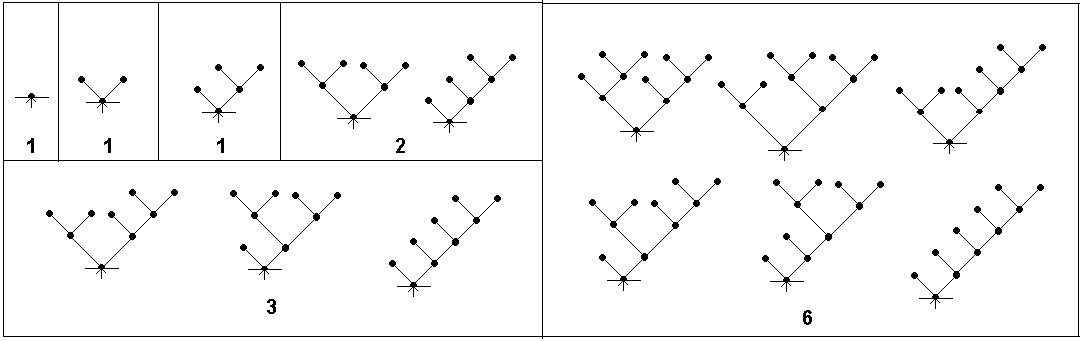
\includegraphics[scale =0.45]{a001190.png}
   \caption{The isomorphic trees for $n=0,1,..., 5$ by \url{https://oeis.org/A001190/a001190.gif}.}
   \label{fig:isotree}
   \end{center}
   \end{figure}
\end{lem}   
                             
\begin{quest}\label{que:hitnum}
For a non-trivial binary tree $T$ and $F(T) \in \Smusati{\delta=1}=\Uclashi{\delta=1}$, is the number of 1-singular variables in $F(T)$ equal $2^{\hts(T)-1}$?
\end{quest}

Some general remarks: 
  \begin{enumerate}
  \item There are exactly two full clause-sets of $\Musati{\delta=1}$, namely $A_0$ and $A_1$.
  \item If a Horn clause-set $F$ (a clause-set with at most one positive literal in each clause) is minimally unsatisfiable, then $F \in \Musati{\delta=1}$.
  \end{enumerate} 
%-----------------------------------------------------------------------------
\subsection{Structure of $\Musati{\delta=2}$}
\label{sec:smu2}

\begin{lem}\label{lem:mu2-mup}
If $F \in \Musati{\delta=2}$ and there is at least one singular variable $v \in \var(F)$, then by an iterated application of singular DP-reduction we get $F' \in \Musatnsi{\delta=2}$.
\end{lem}
\begin{prf}
See Lemma \ref{lem:sDP-infl}.
\end{prf}

\begin{lem}\label{lem:mu2-Fn}
\cite{KleineBuening2000SubclassesMU} If $F \in \Musatnsi{\delta=2}$, then it is in the form of (isomorphism) $\Dt{n}$  for $n \ge 2$ as follows:
  \begin{displaymath}
    \Dt{n} := \set{\set{x_1,\dots,x_n},\set{\ol x_1,\dots,\ol x_n},\set{\ol x_1,x_2}, \dots, \set{\ol x_{n-1},x_n}, \set{\ol x_n,x_1}}.
  \end{displaymath}

\end{lem}
Remarks:
  \begin{enumerate}
  \item According to \cite{KullmannZhao2010Extremal}
  \begin{enumerate}
  \item The only hitting clause-sets amongst the $\Dt{n}$ ($\Uclashnsi{\delta=2}$) are for $n=2,3$. 
  \item All $\Dt{n}$ are saturated, thus $\Musatnsi{\delta=2} = \Smusatnsi{\delta=2}$. Also we have $\minvdeg(\Dt{n}) = 4$. 
  \item $\Dt{n}$ contains two full clauses (one with only positive literals and one with only negative literals) and the rest of clauses are as a cycle $v_1 \ra \dots \ra v_n \ra v_1$ (that at least one variable must be true and one must be false).
  \item By splitting $\Dt{n}$ to $F_0, F_1$ for any variable $v \in \var(\Dt{n})$, we have $F_0, F_1 \in \Musati{\delta=1} $.
  \end{enumerate} 
  \end{enumerate} 
  
\begin{lem}\label{lem:mu2-smu2}
Consider $\Dt{n}$ in Lemma \ref{lem:mu2-Fn}. If we split $\Dt{n}$ to $F_0:=\pao v0 * \Dt{n}$ and $F_1:=\pao v1 * \Dt{n}$ on any variable $v \in \var(\Dt{n})$, then they are not saturated.($F \in \Musatnsi{\delta=2} = \Smusatnsi{\delta=2}$)
\end{lem}
\begin{prf}
Based on Lemma \ref{lem:mu1-sma-uhit}, we have $\Smusati{\delta=1} = \Uclashi{\delta=1}$. Also, since $\Dt{n}$ for $n \ge 4$ is not in $\Uclash$ thus there exists some partial assignment $\vp$ such that $\vp * \Dt{n} \not \in \Musat$. Now, suppose that for all one-variable assignments the result would be in $\Smusati{\delta=1}$. Thus, they would be in $\Uclashi{\delta=1}$, which is stable under partial assignments, and as a result all applications of partial assignments to $\Dt{n}$ would stay in $\Musat$. This yields a contradiction. Since  the literals in $\Dt{n}$ have complete symmetry, thus for $n \ge 4$ no single assignment can yield an element of $\Musati{\delta=1}$.
\end{prf}

\begin{lem}\label{lem:mu2-horn-tree}
Consider splitting $\Dt{n}$ based on Lemma \ref{lem:mu2-smu2} on any variable $v \in \var(\Dt{n})$. Then, $ F_1$ is a Horn clause-set and $ F_0$ is a dual-Horn clause-set. Also, there exist a resolution tree $T$ for $ F_0,F_1$ such that $\hts(T(F_0))= \hts(T(F_1)) \le 1$.
\end{lem}
\begin{prf}
If we split $\Dt{n}$ regarding $x_1$, we have:
\begin{displaymath}
F_0=\set{\set{x_2,\dots,x_n},\set{\ol x_2,x_3},\dots, \set{\ol x_{n-1},x_n},\set{\ol x_n}}.
\end{displaymath}
\begin{displaymath}
F_1=\set{\set{\ol x_2,\dots,\ol x_n},\set{x_2},\set{\ol x_2,x_3}\dots, \set{\ol x_{n-1},x_n}}.
\end{displaymath}
As it can be seen, $F_1$ is a Horn clause-set. Also, if we flip (change the sign) all literals $x$ in  $F_0$ to get $F_0'$, then $F_0'$ is a Horn clause-set and thus, $ F_0$ is a dual-Horn clause-set. Since $\Dt{n}$ have complete symmetry regarding the literals, $F_0, F_1$ for all literals hold these properties. Also, for all Horn clause-sets (and dual-Horn clause-sets) there exist a resolution tree such that $\hts(T) \le 1$.
\end{prf}

\begin{quest}\label{que:mu-2-horn}
If we saturate $F_0, F_1$ in Lemma \ref{lem:mu2-horn-tree}, what would happen to the resolution trees $T(F_0), T(F_1)$ with $\hts(T(F_0))= \hts(T(F_1)) \le 1$?
\end{quest}

\begin{lem}\label{lem:mu2-build}
All $F \in \Musati{\delta=2}$ can be obtained from $\Dt{n}$ (in Lemma \ref{lem:mu2-Fn}) by singular extension of  $\Dt{n}$. Also, for a clause-set $F \in \Musati{\delta=2}$ we can obtain a clause-set $F' \in \Musati{\delta=2}$ via singular extension.
\end{lem}
\begin{prf}
For the first part, consider $F \in \Musati{\delta=2}$. Then, based on Lemma \ref{lem:mu2-Fn} an iterated application of singular DP-reduction leads to $F'=\Dt{n}$. Also, the singular DP-extension is the reverse direction of singular DP-reduction (and does not change the deficiency and minimal unsatisfiability). Thus, we can obtain all $F \in \Musati{\delta=2}$ by singular extension of $\Dt{n}$. For the second part, consider $F \in \Musati{\delta=2}$. Based on definition \ref{def:singularextn}, if $F'$ is obtained by application of singular extension then $F' \in \Musati{\delta=2}$.
\end{prf}
Remarks:
  \begin{enumerate}
  \item There is exactly one full element of $\Musati{\delta=2}$, namely $A_2$.
  \item For $\Dt{n} \in \Smusatnsi{\delta=2}$ and each $v \in \var(\Dt{n})$, $\ve \in \set{0,1}$, holds $\pao v{\ve} * \Dt{n} \in \Musati{\delta=1}$ (by Lemma \ref{lem:smu-mu}).
  \end{enumerate}
  
\begin{lem}\label{lem:mu2-sing}
 By Lemma 5.13 in \cite{KullmannZhao2010Extremal}, if $F \in \Musati{\delta=2}$ with $\minvdeg(F) \ge 4$ then $F$ is singular if and only if $F$ contains a unit-clause.
\end{lem}  

\begin{quest}\label{que:mu-2-ism}
If we extend some of clause-sets in $\Dt{n}$ with different $n$ using Lemma \ref{lem:mu2-build}, is it possible to obtain isomorphic clause-sets with different $n$?
\end{quest}

\begin{quest}\label{que:mu2-from-mu1}
Is every element of $\Musati{\delta=2}$ obtained from some $\Dt{n}$, by expanding every clause via variable-disjoint elements from $\Musati{\delta=1}$ ?
\end{quest}

\begin{quest}\label{que:mu2-uhit2}
How can we describe the subclasses $\Uclashi{\delta=2}$ and $\Smusati{\delta=2}$?
\end{quest}

\begin{quest}\label{que:mu2-hardness}
Based on Section \ref{sec:Hardnessmeasures}, how can we determine the hardness and the width hardness for $F \in \Musati{\delta=2}$? and moreover how can we determine the resolution- and tree-resolution-complexity precisely?
\end{quest}

\begin{quest}\label{que:mu2-count}
Can we count the number of non-isomorphic elements of $F \in \Musati{\delta=2}$ for a given number of clauses?
\end{quest}

%-----------------------------------------------------------------------------
\subsection{Structure of $\Musat$ with $\delta \ge 3$}
\label{sec:smu3}

So far, we discussed the structure of $\Musati{\delta=1}$ in Section \ref{sec:smu1}. Also, for $\Musati{\delta=2}$ in Section \ref{sec:smu2} we showed that by applying singular DP-reduction we get $F \in \Musatnsi{\delta=2}$ (which is in the form of $\Dt{n} $) and then, by splitting we get the elements of $\Musati{\delta=1}$ (which are well-known). In this section, we discuss some properties and questions regarding $F \in \Musat$ with $\delta \ge 3$ for future work.
%The knowledge for the structure of clause-sets in $\Musati{\delta \ge 3}$ is very limited. For example, \cite{KullmannZhao2016UHitSAT} studies the characterization of clause-sets in $\Uclashi{\delta=2} \subset \Musati{\delta=2}$ and \cite{KullmannZhao2010Extremal} investigates some properties of clause-sets with deficiency three. Thus, characterization of clause-sets in this subclass is an open research question.
\begin{lem}\label{lem:muk-k}
By \cite{Ku99dK} if $F \in \Musati{\delta=k}$, then there exist a variable with at most $k$ positive and $k$ negative occurrence. %Lemma C2
\end{lem}

\begin{lem}\label{lem:mu2tomu3}
For any non-full $F \in \Musati{\delta=2}$ ($F \not = A_2$), if we perform a strict full subsumption extension, we can obtain an special group of clause-sets $F' \in \Musati{\delta=3}$. Also, by Definition \ref{def:fse} $F'$ can be obtained by performing a strict full subsumption resolution for $F$.
\end{lem}
\begin{prf}
For $F, F' \in \Cls$ consider $ F' \tsubres F$. Based on Section \ref{sec:fsr-e}, the strict full subsumption extension is the reverse direction of the  strict full subsumption resolution and if $F' \in \Musat$ then we have $F \in \Musat$ (minimal unsatisfiability is stable under the strict full subsumption extension). Also, consider a clause $R \in F$ such that $ x \in \lit(F)$ and $x, \ol x \not \in \lit(R)$. To perform the strict full subsumption extension for $F$, we have $C = R \addcup \set{x}$, $D = R \addcup \set{\ol{x}}, F = (F' \sm \set{R}) \addcup \set{C,D}$. Also, since the operation is strict, the literals $x, \ol x$ must occur in $F \sm \set{R}$ and we have $c(F)=c(F')+1$, $n(F)=n(F')$ and $\delta(F')=3$. Thus, $F' \in \Musati{\delta=3}$.

\end{prf}
Remarks:
\begin{enumerate}
\item If $F$ is saturated/hitting, then so is $F'$. It shouldn't matter which clause of $\Dt{n}$ is chosen for the extension, and thus we obtain here one family $(\Dt{n}')_{n \in \NN, n \ge 3}$ of nonsingular and also saturated elements.
\item If $F$ is nonsingular, so is $F'$, but possibly also for singular $F$ we obtain nonsingular $F'$ (analysis is needed); this yields further examples (also via singular DP-reduction).
\end{enumerate}

\begin{conj}\label{con:mudelta}
By Conjecture 15.6 in \cite{KullmannZhao2010Extremal} for every deficiency $k \in \NN$ there are finitely many ``patterns'' which explain the elements of $\Musatnsi{\delta=k}$, as well as the saturated and hitting cases amongst them.
\end{conj}
 
\begin{quest}\label{que:str-3}
Based on Conjecture \ref{con:mudelta}, is there any isomorphic form for $F \in \Musati{\delta=3}$?
\end{quest}

\begin{quest}\label{que:smu-3}
How can we determine the non-isomorphic elements of $\Uclashnsi{\delta=3}$ and also $\Smusatnsi{\delta=3}$?
\end{quest}
%%%%%%%%%%%%%%%%%%%%%%%%%%%%%%%%%%%%%%%%%%%%%%%%%%%%%%%%%%
\chapter{Research ideas}
\label{cha:concl}

In this????????


  \begin{enumerate}
  \item Question \ref{}: 
  \end{enumerate}
%%%%%%%%%%%%%%%%%%%%%%%%%%%%%%%%%%%%%%%%%%%%%%%%%%%%%%%%%%
%\newpage
\bibliographystyle{plainurl}
%\BibliographyOKlibrary
\bibliography{HA_ResearchRef}

\end{document}

